\documentclass[12pt,]{book}
\usepackage{lmodern}
\usepackage{amssymb,amsmath}
\usepackage{ifxetex,ifluatex}
\usepackage{fixltx2e} % provides \textsubscript
\ifnum 0\ifxetex 1\fi\ifluatex 1\fi=0 % if pdftex
  \usepackage[T1]{fontenc}
  \usepackage[utf8]{inputenc}
\else % if luatex or xelatex
  \ifxetex
    \usepackage{mathspec}
  \else
    \usepackage{fontspec}
  \fi
  \defaultfontfeatures{Ligatures=TeX,Scale=MatchLowercase}
\fi
% use upquote if available, for straight quotes in verbatim environments
\IfFileExists{upquote.sty}{\usepackage{upquote}}{}
% use microtype if available
\IfFileExists{microtype.sty}{%
\usepackage{microtype}
\UseMicrotypeSet[protrusion]{basicmath} % disable protrusion for tt fonts
}{}
\usepackage[margin = 1.2in]{geometry}
\usepackage{hyperref}
\PassOptionsToPackage{usenames,dvipsnames}{color} % color is loaded by hyperref
\hypersetup{unicode=true,
            pdftitle={Tutorial showcasing the cerUB package for R},
            colorlinks=true,
            linkcolor=Maroon,
            citecolor=Blue,
            urlcolor=blue,
            breaklinks=true}
\urlstyle{same}  % don't use monospace font for urls
\usepackage{color}
\usepackage{fancyvrb}
\newcommand{\VerbBar}{|}
\newcommand{\VERB}{\Verb[commandchars=\\\{\}]}
\DefineVerbatimEnvironment{Highlighting}{Verbatim}{commandchars=\\\{\}}
% Add ',fontsize=\small' for more characters per line
\usepackage{framed}
\definecolor{shadecolor}{RGB}{248,248,248}
\newenvironment{Shaded}{\begin{snugshade}}{\end{snugshade}}
\newcommand{\AlertTok}[1]{\textcolor[rgb]{0.94,0.16,0.16}{#1}}
\newcommand{\AnnotationTok}[1]{\textcolor[rgb]{0.56,0.35,0.01}{\textbf{\textit{#1}}}}
\newcommand{\AttributeTok}[1]{\textcolor[rgb]{0.77,0.63,0.00}{#1}}
\newcommand{\BaseNTok}[1]{\textcolor[rgb]{0.00,0.00,0.81}{#1}}
\newcommand{\BuiltInTok}[1]{#1}
\newcommand{\CharTok}[1]{\textcolor[rgb]{0.31,0.60,0.02}{#1}}
\newcommand{\CommentTok}[1]{\textcolor[rgb]{0.56,0.35,0.01}{\textit{#1}}}
\newcommand{\CommentVarTok}[1]{\textcolor[rgb]{0.56,0.35,0.01}{\textbf{\textit{#1}}}}
\newcommand{\ConstantTok}[1]{\textcolor[rgb]{0.00,0.00,0.00}{#1}}
\newcommand{\ControlFlowTok}[1]{\textcolor[rgb]{0.13,0.29,0.53}{\textbf{#1}}}
\newcommand{\DataTypeTok}[1]{\textcolor[rgb]{0.13,0.29,0.53}{#1}}
\newcommand{\DecValTok}[1]{\textcolor[rgb]{0.00,0.00,0.81}{#1}}
\newcommand{\DocumentationTok}[1]{\textcolor[rgb]{0.56,0.35,0.01}{\textbf{\textit{#1}}}}
\newcommand{\ErrorTok}[1]{\textcolor[rgb]{0.64,0.00,0.00}{\textbf{#1}}}
\newcommand{\ExtensionTok}[1]{#1}
\newcommand{\FloatTok}[1]{\textcolor[rgb]{0.00,0.00,0.81}{#1}}
\newcommand{\FunctionTok}[1]{\textcolor[rgb]{0.00,0.00,0.00}{#1}}
\newcommand{\ImportTok}[1]{#1}
\newcommand{\InformationTok}[1]{\textcolor[rgb]{0.56,0.35,0.01}{\textbf{\textit{#1}}}}
\newcommand{\KeywordTok}[1]{\textcolor[rgb]{0.13,0.29,0.53}{\textbf{#1}}}
\newcommand{\NormalTok}[1]{#1}
\newcommand{\OperatorTok}[1]{\textcolor[rgb]{0.81,0.36,0.00}{\textbf{#1}}}
\newcommand{\OtherTok}[1]{\textcolor[rgb]{0.56,0.35,0.01}{#1}}
\newcommand{\PreprocessorTok}[1]{\textcolor[rgb]{0.56,0.35,0.01}{\textit{#1}}}
\newcommand{\RegionMarkerTok}[1]{#1}
\newcommand{\SpecialCharTok}[1]{\textcolor[rgb]{0.00,0.00,0.00}{#1}}
\newcommand{\SpecialStringTok}[1]{\textcolor[rgb]{0.31,0.60,0.02}{#1}}
\newcommand{\StringTok}[1]{\textcolor[rgb]{0.31,0.60,0.02}{#1}}
\newcommand{\VariableTok}[1]{\textcolor[rgb]{0.00,0.00,0.00}{#1}}
\newcommand{\VerbatimStringTok}[1]{\textcolor[rgb]{0.31,0.60,0.02}{#1}}
\newcommand{\WarningTok}[1]{\textcolor[rgb]{0.56,0.35,0.01}{\textbf{\textit{#1}}}}
\usepackage{longtable,booktabs}
\usepackage{graphicx,grffile}
\makeatletter
\def\maxwidth{\ifdim\Gin@nat@width>\linewidth\linewidth\else\Gin@nat@width\fi}
\def\maxheight{\ifdim\Gin@nat@height>\textheight\textheight\else\Gin@nat@height\fi}
\makeatother
% Scale images if necessary, so that they will not overflow the page
% margins by default, and it is still possible to overwrite the defaults
% using explicit options in \includegraphics[width, height, ...]{}
\setkeys{Gin}{width=\maxwidth,height=\maxheight,keepaspectratio}
\IfFileExists{parskip.sty}{%
\usepackage{parskip}
}{% else
\setlength{\parindent}{0pt}
\setlength{\parskip}{6pt plus 2pt minus 1pt}
}
\setlength{\emergencystretch}{3em}  % prevent overfull lines
\providecommand{\tightlist}{%
  \setlength{\itemsep}{0pt}\setlength{\parskip}{0pt}}
\setcounter{secnumdepth}{5}
% Redefines (sub)paragraphs to behave more like sections
\ifx\paragraph\undefined\else
\let\oldparagraph\paragraph
\renewcommand{\paragraph}[1]{\oldparagraph{#1}\mbox{}}
\fi
\ifx\subparagraph\undefined\else
\let\oldsubparagraph\subparagraph
\renewcommand{\subparagraph}[1]{\oldsubparagraph{#1}\mbox{}}
\fi

%%% Use protect on footnotes to avoid problems with footnotes in titles
\let\rmarkdownfootnote\footnote%
\def\footnote{\protect\rmarkdownfootnote}

%%% Change title format to be more compact
\usepackage{titling}

% Create subtitle command for use in maketitle
\providecommand{\subtitle}[1]{
  \posttitle{
    \begin{center}\large#1\end{center}
    }
}

\setlength{\droptitle}{-2em}

  \title{Tutorial showcasing the cerUB package for R}
    \pretitle{\vspace{\droptitle}\centering\huge}
  \posttitle{\par}
    \author{}
    \preauthor{}\postauthor{}
      \predate{\centering\large\emph}
  \postdate{\par}
    \date{2019-09-24}

\usepackage{setspace}
\usepackage{chngcntr}
\usepackage{microtype}
\usepackage{fancyhdr}
\usepackage{placeins}
\usepackage{booktabs}
\usepackage{amsthm}
\makeatletter
\def\thm@space@setup{%
  \thm@preskip=8pt plus 2pt minus 4pt
  \thm@postskip=\thm@preskip
}
\makeatother

\begin{document}
\maketitle

{
\hypersetup{linkcolor=black}
\setcounter{tocdepth}{1}
\tableofcontents
}
\hypertarget{cerub-tutorial}{%
\chapter*{cerUB tutorial}\label{cerub-tutorial}}
\addcontentsline{toc}{chapter}{cerUB tutorial}

Tutorial showcasing the cerUB package for R (\href{https://github.com/Andros-Spica/cerUB}{cerUB}).

This document shows how to use \emph{cerUB} protocols to explore petrographic and compositional data. As an example, we provide the `amphorae' dataset concerning wine Roman amphorae from sites in Catalonia, NE Spain. It is a live version of the Appendix C of an article published in Journal of Archaeological Science (see reference below).

\begin{enumerate}
\def\labelenumi{\arabic{enumi}.}
\tightlist
\item
  \protect\hyperlink{install}{Installing cerUB}
\item
  \protect\hyperlink{init}{Initial procedures}
\item
  \protect\hyperlink{prot1}{Protocol 1 - Geochemical data}
\item
  \protect\hyperlink{prot2}{Protocol 2 - Petrographic data}
\item
  \protect\hyperlink{prot3}{Protocol 3 - Geochemical and petrographic data}
\item
  \protect\hyperlink{prot4}{Protocol 4 - Provenance data}
\item
  \protect\hyperlink{prot4_ship}{Protocol 4 - Provenance data with shipwrecks}
\item
  \protect\hyperlink{interp_biplots}{Appendix: Interpreting biplots}
\end{enumerate}

\begin{center}\rule{0.5\linewidth}{\linethickness}\end{center}

All rmarkdown (.Rmd) source files are available in the \href{https://github.com/Andros-Spica/cerUB_tutorial}{repository}.

There, the \href{https://github.com/Andros-Spica/cerUB_tutorial/tree/master/publication_appendices}{publication appendices} folder contains alternative versions of the appendices (supplementary materials) of the related article:

\begin{quote}
Angourakis, A., Martínez Ferreras, V., Torrano A., Gurt Esparraguera, J.M. (2018) Presenting multivariate statistical protocols in R using Roman wine amphorae productions in Catalonia, Spain. \emph{Journal of Archaeological Science}, 93:150-165. \url{https://doi.org/10.1016/j.jas.2018.03.007}
\end{quote}

Additionaly, the repository also contains:
- \href{https://github.com/Andros-Spica/cerUB_tutorial/blob/master/poster_ISA2018/ISA2018_Angourakis_et_al.pdf}{Poster} presented in the International Symposium on Archaeometry (ISA) in Merida, Mexico, May 2018.
- \href{https://github.com/Andros-Spica/cerUB_tutorial/tree/master/poster_OpenScienceHumanities2018/OSH2018_Angourakis_et_al.pdf}{Poster} presented in the Open Science and The Humanities Conference in Barcelona, Spain, June 2018.

Please, address any issues, suggestions, and comments to Andreas Angourakis (\href{mailto:andros.spica@gmail.com}{\nolinkurl{andros.spica@gmail.com}}, or through \emph{GitHub}, user \textbf{Andros-Spica})

\hypertarget{install}{%
\chapter{Installing cerUB}\label{install}}

There are two options for installing the \emph{cerUB} package:

\begin{enumerate}
\def\labelenumi{\alph{enumi}.}
\tightlist
\item
  Downloading the latest release version from \href{zenodo.org}{Zenodo.org} and installing it in \href{rstudio.com}{RStudio} (Tools \textgreater{} Install Packages\ldots{} \textgreater{} Install from: Package Archive File).
\end{enumerate}

\begin{quote}
Angourakis, Andreas, \& Martínez Ferreras, Verònica. (2017, September 23). cerUB - Protocols for exploring archaeometric data (R package). Zenodo. \url{http://doi.org/10.5281/zenodo.975451}
\end{quote}

\begin{enumerate}
\def\labelenumi{\alph{enumi}.}
\setcounter{enumi}{1}
\tightlist
\item
  Installing the latest development version directly from \href{github.com}{GitHub} (\href{https://github.com/Andros-Spica/cerUB}{Andros-Spica/cerUB}), using the \emph{devtools} package:
\end{enumerate}

\begin{Shaded}
\begin{Highlighting}[]
\CommentTok{# this will install devtools package, if not installed already}
\ControlFlowTok{if}\NormalTok{ (}\OperatorTok{!}\KeywordTok{require}\NormalTok{(}\StringTok{"devtools"}\NormalTok{))}
    \KeywordTok{install.packages}\NormalTok{(}\StringTok{"devtools"}\NormalTok{) }

\NormalTok{devtools}\OperatorTok{::}\KeywordTok{install_github}\NormalTok{(}\StringTok{"Andros-Spica/cerUB"}\NormalTok{)}
\end{Highlighting}
\end{Shaded}

The second option is recommended, because it is a faster way to install and update packages that are not in \href{cran.r-project.org}{CRAN}.

The same options are available for installing the \emph{biplot2d3d} package, which we use here to plot protocols results.

\begin{quote}
Andreas Angourakis. (2017, September 20). biplot2d3d - an R package for generating highly-customizable biplots. Zenodo. \url{http://doi.org/10.5281/zenodo.897603}
\end{quote}

\begin{Shaded}
\begin{Highlighting}[]
\NormalTok{devtools}\OperatorTok{::}\KeywordTok{install_github}\NormalTok{(}\StringTok{"Andros-Spica/biplot2d3d"}\NormalTok{)}
\end{Highlighting}
\end{Shaded}

Any other package required by these two packages (\emph{ade4}, \emph{rgl}, etc.) should be automatically installed.

\hypertarget{init}{%
\chapter{Initial procedures}\label{init}}

Load \emph{cerUB} package.

\begin{Shaded}
\begin{Highlighting}[]
\KeywordTok{library}\NormalTok{(cerUB)}
\end{Highlighting}
\end{Shaded}

\hypertarget{set-directories-for-saving-data}{%
\section{Set directories for saving data}\label{set-directories-for-saving-data}}

Set a list containing directories for easiness of reference:

\begin{Shaded}
\begin{Highlighting}[]
\NormalTok{directories <-}\StringTok{ }\KeywordTok{list}\NormalTok{(}
  \CommentTok{# where you raw data is}
  \DataTypeTok{data =} \StringTok{"data"}\NormalTok{, }
  \CommentTok{# where to save transformed compositional data (CoDa)}
  \DataTypeTok{transCoDa =} \StringTok{"transformed_CoDa"}\NormalTok{, }
  \CommentTok{# where to save files concerning protocol workflow}
  \DataTypeTok{prot1 =} \StringTok{"Protocol_1_geochemical_data"}\NormalTok{,}
  \DataTypeTok{prot2 =} \StringTok{"Protocol_2_petrographic_data"}\NormalTok{,}
  \DataTypeTok{prot3 =} \StringTok{"Protocol_3_geochemical_and_petrographic_data"}\NormalTok{,}
  \DataTypeTok{prot4 =} \StringTok{"Protocol_4_provenance_data"}\NormalTok{,}
  \DataTypeTok{prot4_Shipwreck =} \StringTok{"Protocols_4_provenance_data_with_shipwrecks"}
\NormalTok{)}
\end{Highlighting}
\end{Shaded}

Create the respective folders in the current R session working directory, if they do not exist:

\begin{Shaded}
\begin{Highlighting}[]
\KeywordTok{lapply}\NormalTok{(directories, dir.create, }\DataTypeTok{showWarnings =} \OtherTok{FALSE}\NormalTok{)}
\end{Highlighting}
\end{Shaded}

\hypertarget{read-data}{%
\section{Read data}\label{read-data}}

Load the amphorae dataset:

\begin{Shaded}
\begin{Highlighting}[]
\KeywordTok{data}\NormalTok{(amphorae)}
\end{Highlighting}
\end{Shaded}

Or, alternatively, your own dataset (e.g., CSV):

\begin{Shaded}
\begin{Highlighting}[]
\NormalTok{dt <-}\StringTok{ }\KeywordTok{cbind}\NormalTok{(}\KeywordTok{read.csv}\NormalTok{(}\KeywordTok{paste}\NormalTok{(directories}\OperatorTok{$}\NormalTok{data,}
                           \StringTok{"petrographic_data.csv"}\NormalTok{,}\DataTypeTok{sep=}\StringTok{"/"}\NormalTok{),}
                     \CommentTok{# assuming the first column contains row names}
                     \DataTypeTok{row.names=}\DecValTok{1}\NormalTok{), }
            \KeywordTok{read.csv}\NormalTok{(}\KeywordTok{paste}\NormalTok{(directories}\OperatorTok{$}\NormalTok{data,}
                           \StringTok{"geochemical_data.csv"}\NormalTok{,}\DataTypeTok{sep=}\StringTok{"/"}\NormalTok{),}
                     \CommentTok{# assuming the first column contains row names}
                     \DataTypeTok{row.names=}\DecValTok{1}\NormalTok{)) }
\end{Highlighting}
\end{Shaded}

Note that if you use your own dataset you must replace all references to ``amphorae'' with your data frame name (e.g.~``dt'').

\hypertarget{codify-petrographical-variables}{%
\section{Codify petrographical variables}\label{codify-petrographical-variables}}

Create a two-column data frame containing the original names of petrographic variables and their respective codes:

\begin{Shaded}
\begin{Highlighting}[]
\NormalTok{varCode <-}\StringTok{ }\KeywordTok{code_variables}\NormalTok{(amphorae)}
\end{Highlighting}
\end{Shaded}

Petrographic variables must be named following \emph{cerUB} naming system. Consult the documentation on the ``amphorae'' dataset by running:

\begin{Shaded}
\begin{Highlighting}[]
\NormalTok{?amphorae}
\end{Highlighting}
\end{Shaded}

The result of the \textbf{code\_variables} function is used in the \textbf{apply\_ordination} function for protocols ``2a'', ``2b'', ``3'', and ``4'' (i.e., whenever there are ordinal input variables). The data frame containing the codification (`varCode') is attached as ``ordination\_object\$variable\_tags'' to the resulting ordination object.

\begin{tabular}{l|l}
\hline
Variable name & Variable code\\
\hline
Site\_Name & Site\_Name\\
\hline
LOCATION\_SITE\_INITIALS & LOCATION\_SITE\_INITIALS\\
\hline
CHARAC & CHARAC\\
\hline
FabricGroup & FabricGroup\\
\hline
ChemReferenceGroup & ChemReferenceGroup\\
\hline
INCLUS\_DISTRIB & I1\\
\hline
INCLUS\_ORIENT & I2\\
\hline
TEMP & F1\\
\hline
ATM & F2\\
\hline
POST\_ATM & F3\\
\hline
VOID\_OVERALL & V1\\
\hline
VOID\_VESIC\_MEGA & V2\\
\hline
... & ...\\
\hline
\end{tabular}

\hypertarget{clean-and-format-data}{%
\section{Clean and format data}\label{clean-and-format-data}}

Cleaning and format procedures, including coercing variables as numeric or factor, excluding columns (constants, perturbed, unreliable) and rows (incomplete data, outliers).

\begin{Shaded}
\begin{Highlighting}[]
\NormalTok{cleanAmphorae <-}\StringTok{ }\KeywordTok{clean_and_format}\NormalTok{(}
\NormalTok{  amphorae,}
  \DataTypeTok{completion_variable =} \KeywordTok{c}\NormalTok{(}
    \CommentTok{# The variable with completion info}
    \StringTok{"CHARAC"}\NormalTok{, }
    \CommentTok{# the value indicating completion}
    \StringTok{"complete"}
\NormalTok{  ), }
  \DataTypeTok{categorical_columns =} \DecValTok{1}\OperatorTok{:}\DecValTok{112}\NormalTok{, }
  \DataTypeTok{numerical_columns =} \DecValTok{113}\OperatorTok{:}\KeywordTok{ncol}\NormalTok{(amphorae),}
  \CommentTok{# values converted to NA}
  \DataTypeTok{as_na =} \KeywordTok{c}\NormalTok{(}\StringTok{"NULL"}\NormalTok{, }\StringTok{"indeterminate"}\NormalTok{, }\StringTok{"unfired"}\NormalTok{),}
  \CommentTok{# method for replacing NAs}
  \DataTypeTok{method =} \OtherTok{NULL}\NormalTok{, }
  \CommentTok{# don't use the following variables}
  \DataTypeTok{columns_to_exclude =} \KeywordTok{c}\NormalTok{(}\StringTok{"VOID_VESIC_MEGA"}\NormalTok{, }\StringTok{"VOID_VUGH_MEGA"}\NormalTok{,}
                         \StringTok{"VOID_CHAN_MEGA"}\NormalTok{, }\StringTok{"VOID_PLAN_MEGA"}\NormalTok{,}
                         \StringTok{"COAR_R_DAC_AND"}\NormalTok{, }\StringTok{"COAR_R_EVAP"}\NormalTok{,}
                         \StringTok{"COAR_R_CONGBREC"}\NormalTok{, }\StringTok{"COAR_R_SERP"}\NormalTok{,}
                         \StringTok{"COAR_C_SPL"}\NormalTok{, }\StringTok{"COAR_C_OPX"}\NormalTok{,}
                         \StringTok{"COAR_C_OL"}\NormalTok{, }\StringTok{"COAR_C_SIL"}\NormalTok{,}
                         \StringTok{"COAR_C_ST"}\NormalTok{, }\StringTok{"COAR_C_ZRN"}\NormalTok{,}
                         \StringTok{"COAR_C_PY"}\NormalTok{, }\StringTok{"FINE_C_OPX"}\NormalTok{,}
                         \StringTok{"FINE_C_ZRN"}\NormalTok{),}
  \CommentTok{# don't use the following observations}
  \CommentTok{# (Italic amphorae from Port Vendres 4)}
  \DataTypeTok{rows_to_exclude =} \KeywordTok{c}\NormalTok{(}\StringTok{"PV4033"}\NormalTok{, }\CommentTok{# PV4-IND4}
                      \StringTok{"PV4017"}\NormalTok{, }\CommentTok{# PV4-CAMP}
                      \CommentTok{# PV4-ITT}
                      \StringTok{"PV4021"}\NormalTok{, }\StringTok{"PV4023"}\NormalTok{, }\StringTok{"PV4024"}\NormalTok{, }
                      \StringTok{"PV4025"}\NormalTok{, }\StringTok{"PV4035"}\NormalTok{, }\StringTok{"PV4037"}\NormalTok{,}
                      \CommentTok{# PV4-NAP}
                      \StringTok{"PV4022"}\NormalTok{, }\StringTok{"PV4026"}\NormalTok{, }\StringTok{"PV4027"}\NormalTok{, }
                      \StringTok{"PV4028"}\NormalTok{, }\StringTok{"PV4029"}\NormalTok{, }\StringTok{"PV4030"}\NormalTok{,}
                      \StringTok{"PV4036"}\NormalTok{)}
\NormalTok{)}
\end{Highlighting}
\end{Shaded}

\begin{tabular}{l|l|l}
\hline
  & Variables & Observations\\
\hline
amphorae & 138 & 238\\
\hline
cleanAmphorae & 91 & 223\\
\hline
\end{tabular}

\hypertarget{subsetting-criteria}{%
\section{Subsetting criteria}\label{subsetting-criteria}}

Build vector indicating whether each observation is from a shipwreck:

\begin{Shaded}
\begin{Highlighting}[]
\NormalTok{isShipwreck <-}
\StringTok{  }\NormalTok{cleanAmphorae}\OperatorTok{$}\NormalTok{Site_Name}\OperatorTok{==}\StringTok{"Cap del Vol"} \OperatorTok{|}
\StringTok{  }\NormalTok{cleanAmphorae}\OperatorTok{$}\NormalTok{Site_Name}\OperatorTok{==}\StringTok{"Ullastres I"} \OperatorTok{|}
\StringTok{  }\NormalTok{cleanAmphorae}\OperatorTok{$}\NormalTok{Site_Name}\OperatorTok{==}\StringTok{"Port-Vendres 4"}
\end{Highlighting}
\end{Shaded}

\begin{tabular}{l|r|r}
\hline
  & Workshops & Shipwrecks\\
\hline
 & 175 & 48\\
\hline
\end{tabular}

Build vectors indicating provenance group and whether observations are true outliers (IND, observations with no group assigned). Also, reformat ``FabricGroup'' and ``ChemReferenceGroup'', so true outliers are singled out separately and not as a extra group.

\begin{Shaded}
\begin{Highlighting}[]
\NormalTok{ProvenanceGroup <-}\StringTok{ }\KeywordTok{c}\NormalTok{()}
\NormalTok{isTrueIND <-}\StringTok{ }\KeywordTok{c}\NormalTok{()}

\CommentTok{# coerce the original group variables (factors) into character vectors}
\CommentTok{# so we can use stringr package to operate on them.}
\NormalTok{cleanAmphorae}\OperatorTok{$}\NormalTok{FabricGroup <-}\StringTok{ }
\StringTok{  }\KeywordTok{as.character}\NormalTok{(cleanAmphorae}\OperatorTok{$}\NormalTok{FabricGroup)}
\NormalTok{cleanAmphorae}\OperatorTok{$}\NormalTok{ChemReferenceGroup <-}\StringTok{ }
\StringTok{  }\KeywordTok{as.character}\NormalTok{(cleanAmphorae}\OperatorTok{$}\NormalTok{ChemReferenceGroup)}

\ControlFlowTok{for}\NormalTok{ (i }\ControlFlowTok{in} \DecValTok{1}\OperatorTok{:}\KeywordTok{nrow}\NormalTok{(cleanAmphorae))\{}
\NormalTok{  groupChem <-}
\StringTok{    }\NormalTok{stringr}\OperatorTok{::}\KeywordTok{str_split}\NormalTok{(cleanAmphorae}\OperatorTok{$}\NormalTok{ChemReferenceGroup[i], }\StringTok{"-"}\NormalTok{)[[}\DecValTok{1}\NormalTok{]]}
\NormalTok{  groupFabric <-}
\StringTok{    }\NormalTok{stringr}\OperatorTok{::}\KeywordTok{str_split}\NormalTok{(cleanAmphorae}\OperatorTok{$}\NormalTok{FabricGroup[i], }\StringTok{"-"}\NormalTok{)[[}\DecValTok{1}\NormalTok{]]}
\NormalTok{  group <-}\StringTok{ ""}
\NormalTok{  isATrueInd <-}\StringTok{ }\OtherTok{FALSE}

  \ControlFlowTok{if}\NormalTok{ (groupChem[}\DecValTok{2}\NormalTok{] }\OperatorTok{==}\StringTok{ "IND"} \OperatorTok{||}\StringTok{ }\NormalTok{groupFabric[}\DecValTok{2}\NormalTok{] }\OperatorTok{==}\StringTok{ "IND"}\NormalTok{) \{}
\NormalTok{    group <-}\StringTok{ }\NormalTok{cleanAmphorae}\OperatorTok{$}\NormalTok{ChemReferenceGroup[i]}
    \ControlFlowTok{if}\NormalTok{ (}\OperatorTok{!}\NormalTok{isShipwreck[i]) isATrueInd <-}\StringTok{ }\OtherTok{TRUE}
\NormalTok{    index <-}\StringTok{ }\DecValTok{1}
    \ControlFlowTok{for}\NormalTok{ (j }\ControlFlowTok{in} \DecValTok{1}\OperatorTok{:}\KeywordTok{length}\NormalTok{(ProvenanceGroup))\{}
      \ControlFlowTok{if}\NormalTok{ (ProvenanceGroup[j] }\OperatorTok{==}\StringTok{ }\KeywordTok{paste}\NormalTok{(group, index, }\DataTypeTok{sep =} \StringTok{""}\NormalTok{))}
\NormalTok{        index <-}\StringTok{ }\NormalTok{index }\OperatorTok{+}\StringTok{ }\DecValTok{1}
\NormalTok{    \}}
\NormalTok{    group <-}\StringTok{ }\KeywordTok{paste}\NormalTok{(group, index, }\DataTypeTok{sep =} \StringTok{""}\NormalTok{)}
\NormalTok{    cleanAmphorae}\OperatorTok{$}\NormalTok{ChemReferenceGroup[i] <-}\StringTok{ }\NormalTok{group}
\NormalTok{    cleanAmphorae}\OperatorTok{$}\NormalTok{FabricGroup[i] <-}\StringTok{ }\NormalTok{group}
\NormalTok{  \}}
  \ControlFlowTok{else}\NormalTok{ \{}
    \ControlFlowTok{if}\NormalTok{ (groupChem[}\DecValTok{1}\NormalTok{] }\OperatorTok{==}\StringTok{ "ULL"} \OperatorTok{||}\StringTok{ }
\StringTok{        }\NormalTok{groupChem[}\DecValTok{1}\NormalTok{] }\OperatorTok{==}\StringTok{ "PV4"} \OperatorTok{||}\StringTok{ }
\StringTok{        }\NormalTok{groupChem[}\DecValTok{1}\NormalTok{] }\OperatorTok{==}\StringTok{ "CDV"}\NormalTok{) \{}
\NormalTok{      group <-}\StringTok{ }\NormalTok{cleanAmphorae}\OperatorTok{$}\NormalTok{ChemReferenceGroup[i]}
\NormalTok{    \}}
    \ControlFlowTok{else} \ControlFlowTok{if}\NormalTok{ (groupChem[}\DecValTok{1}\NormalTok{] }\OperatorTok{==}\StringTok{ }\NormalTok{groupFabric[}\DecValTok{1}\NormalTok{])\{}
\NormalTok{      group <-}\StringTok{ }\NormalTok{groupChem[}\DecValTok{1}\NormalTok{]}
\NormalTok{    \}}
\NormalTok{  \}}
\NormalTok{  ProvenanceGroup <-}\StringTok{ }\KeywordTok{c}\NormalTok{(ProvenanceGroup, group[}\DecValTok{1}\NormalTok{])}
\NormalTok{  isTrueIND <-}\StringTok{ }\KeywordTok{c}\NormalTok{(isTrueIND, isATrueInd)}
\NormalTok{\}}
\end{Highlighting}
\end{Shaded}

\begin{tabular}{l|r|r}
\hline
  & Assigned & Outliers\\
\hline
 & 205 & 18\\
\hline
\end{tabular}

\hypertarget{organizing-groups}{%
\section{Organizing groups}\label{organizing-groups}}

Build lists of named group factors for easiness of reference.

First, create a list aiming to define workshops productions, so no shipwrecks:

\begin{Shaded}
\begin{Highlighting}[]
\NormalTok{factor_list <-}
\StringTok{  }\KeywordTok{list}\NormalTok{(}
    \DataTypeTok{Site =} \KeywordTok{factor}\NormalTok{(cleanAmphorae}\OperatorTok{$}\NormalTok{Site_Name[}\OperatorTok{!}\NormalTok{isShipwreck]),}
    \DataTypeTok{FabricGroup =} \KeywordTok{factor}\NormalTok{(cleanAmphorae}\OperatorTok{$}\NormalTok{FabricGroup[}\OperatorTok{!}\NormalTok{isShipwreck]),}
    \DataTypeTok{ChemGroup =} \KeywordTok{factor}\NormalTok{(cleanAmphorae}\OperatorTok{$}\NormalTok{ChemReferenceGroup[}\OperatorTok{!}\NormalTok{isShipwreck]),}
    \DataTypeTok{ProvGroup =} \KeywordTok{factor}\NormalTok{(ProvenanceGroup[}\OperatorTok{!}\NormalTok{isShipwreck])}
\NormalTok{  )}
\end{Highlighting}
\end{Shaded}

\begin{tabular}{l|l|l|l|l}
\hline
  & Site & FabricGroup & ChemGroup & ProvGroup\\
\hline
ACM001 & Ca L'Arnau-Can Pau Ferrer & ACM-2 & ACM-C & ACM\\
\hline
ACM097 & Ca L'Arnau-Can Pau Ferrer & ACM-1 & ACM-A & ACM\\
\hline
BIF006 & BDN-Pompeu Fabra & BIF-1 & BIF-2 & BIF\\
\hline
BIF048 & BDN-Pompeu Fabra & BIF-1 & BIF-3 & BIF\\
\hline
CRC002 & Cal Ros de les Cabres & CRC-1 & CRC-1 & CRC\\
\hline
ELV002 & El Vilarenc & ELV-1 & ELV-1 & ELV\\
\hline
ELV051 & El Vilarenc & ELV-1 & ELV-2 & ELV\\
\hline
FEU009 & Can Feu & FEU-IND1 & FEU-IND1 & FEU-IND1\\
\hline
LLA010 & Llafranc & LLA-1 & LLA-A2 & LLA\\
\hline
MOR018 & El More & MOR-2 & MOR-3 & MOR\\
\hline
SAL025 & La Salut & SAL-2 & SAL-1 & SAL\\
\hline
SBL045 & Sant Boi Historic Centre & SBL-2 & SBL-2 & SBL\\
\hline
\end{tabular}

Then, create a second list, aiming to assign shipwreck observations to workshop productions, so with shipwreck samples but no true outliers:

\begin{Shaded}
\begin{Highlighting}[]
\NormalTok{factor_list_Shipwreck <-}
\StringTok{  }\KeywordTok{list}\NormalTok{(}
    \DataTypeTok{Site =} \KeywordTok{factor}\NormalTok{(cleanAmphorae}\OperatorTok{$}\NormalTok{Site_Name[}\OperatorTok{!}\NormalTok{isTrueIND]),}
    \DataTypeTok{FabricGroup =} \KeywordTok{factor}\NormalTok{(cleanAmphorae}\OperatorTok{$}\NormalTok{FabricGroup[}\OperatorTok{!}\NormalTok{isTrueIND]),}
    \DataTypeTok{ChemGroup =} \KeywordTok{factor}\NormalTok{(cleanAmphorae}\OperatorTok{$}\NormalTok{ChemReferenceGroup[}\OperatorTok{!}\NormalTok{isTrueIND]),}
    \DataTypeTok{ProvGroup =} \KeywordTok{factor}\NormalTok{(ProvenanceGroup[}\OperatorTok{!}\NormalTok{isTrueIND])}
\NormalTok{  )}
\end{Highlighting}
\end{Shaded}

\hypertarget{helper-objects-for-plotting}{%
\section{Helper objects for plotting}\label{helper-objects-for-plotting}}

Build lists of named point types vectors for easiness of reference.

Create point type vectors for the whole dataset:

\begin{Shaded}
\begin{Highlighting}[]
\NormalTok{labels_code <-}\StringTok{ }\KeywordTok{as.character}\NormalTok{(}\KeywordTok{row.names}\NormalTok{(cleanAmphorae)) }\CommentTok{# using row names}
\NormalTok{labels_cross <-}\StringTok{ }\KeywordTok{rep}\NormalTok{(}\StringTok{"+"}\NormalTok{, }\KeywordTok{nrow}\NormalTok{(cleanAmphorae)) }\CommentTok{# using +}
\NormalTok{labels_x <-}\StringTok{ }\KeywordTok{rep}\NormalTok{(}\DecValTok{4}\NormalTok{, }\KeywordTok{nrow}\NormalTok{(cleanAmphorae)) }\CommentTok{# using pch code}
\NormalTok{labels_point <-}\StringTok{ }\KeywordTok{rep}\NormalTok{(}\DecValTok{20}\NormalTok{, }\KeywordTok{nrow}\NormalTok{(cleanAmphorae)) }\CommentTok{# using pch code}
\end{Highlighting}
\end{Shaded}

Create a list aiming to define workshops productions:

\begin{Shaded}
\begin{Highlighting}[]
\NormalTok{labels_list <-}\StringTok{ }\KeywordTok{list}\NormalTok{(}
  \DataTypeTok{Code =}\NormalTok{ labels_code[}\OperatorTok{!}\NormalTok{isShipwreck],}
  \DataTypeTok{Cross =}\NormalTok{ labels_cross[}\OperatorTok{!}\NormalTok{isShipwreck],}
  \DataTypeTok{X =}\NormalTok{ labels_x[}\OperatorTok{!}\NormalTok{isShipwreck],}
  \DataTypeTok{Point =}\NormalTok{ labels_point[}\OperatorTok{!}\NormalTok{isShipwreck]}
\NormalTok{)}
\end{Highlighting}
\end{Shaded}

Create a list aiming to assign shipwreck observations to workshop productions:

\begin{Shaded}
\begin{Highlighting}[]
\NormalTok{labels_list_Shipwreck <-}\StringTok{ }\KeywordTok{list}\NormalTok{(}
  \DataTypeTok{Code =}\NormalTok{ labels_code[}\OperatorTok{!}\NormalTok{isTrueIND],}
  \DataTypeTok{Cross =}\NormalTok{ labels_cross[}\OperatorTok{!}\NormalTok{isTrueIND],}
  \DataTypeTok{X =}\NormalTok{ labels_x[}\OperatorTok{!}\NormalTok{isTrueIND],}
  \DataTypeTok{Point =}\NormalTok{ labels_point[}\OperatorTok{!}\NormalTok{isTrueIND]}
\NormalTok{)}
\end{Highlighting}
\end{Shaded}

Build two other lists containing named group color vectors, picking different colors within the \textbf{rainbow} palette:

\begin{Shaded}
\begin{Highlighting}[]
\NormalTok{color_list <-}\StringTok{ }\KeywordTok{list}\NormalTok{()}

\ControlFlowTok{for}\NormalTok{ (i }\ControlFlowTok{in} \DecValTok{1}\OperatorTok{:}\KeywordTok{length}\NormalTok{(factor_list))\{}
\NormalTok{  cv <-}\StringTok{ }\KeywordTok{rainbow}\NormalTok{(}\KeywordTok{nlevels}\NormalTok{(factor_list[[i]]), }\DataTypeTok{v=}\NormalTok{.}\DecValTok{8}\NormalTok{)}
\NormalTok{  color_list[[i]] <-}\StringTok{ }\NormalTok{cv}
  \KeywordTok{names}\NormalTok{(color_list)[i] =}\StringTok{ }\KeywordTok{names}\NormalTok{(factor_list)[i]}
\NormalTok{\}}

\NormalTok{color_list_Shipwreck <-}\StringTok{ }\KeywordTok{list}\NormalTok{()}

\ControlFlowTok{for}\NormalTok{ (i }\ControlFlowTok{in} \DecValTok{1}\OperatorTok{:}\KeywordTok{length}\NormalTok{(factor_list_Shipwreck))\{}
\NormalTok{  cv <-}\StringTok{ }\KeywordTok{rainbow}\NormalTok{(}\KeywordTok{nlevels}\NormalTok{(factor_list_Shipwreck[[i]]), }\DataTypeTok{v=}\NormalTok{.}\DecValTok{8}\NormalTok{)}
\NormalTok{  color_list_Shipwreck[[i]] <-}\StringTok{ }\NormalTok{cv}
  \KeywordTok{names}\NormalTok{(color_list_Shipwreck)[i] =}\StringTok{ }\KeywordTok{names}\NormalTok{(factor_list_Shipwreck)[i]}
\NormalTok{\}}
\end{Highlighting}
\end{Shaded}

To visualize the colors:

\begin{Shaded}
\begin{Highlighting}[]
\KeywordTok{par}\NormalTok{(}\DataTypeTok{mar =} \KeywordTok{c}\NormalTok{(}\DecValTok{0}\NormalTok{,}\DecValTok{0}\NormalTok{,}\DecValTok{0}\NormalTok{,}\DecValTok{0}\NormalTok{))}
\KeywordTok{barplot}\NormalTok{(}\KeywordTok{rep}\NormalTok{(}\DecValTok{100}\NormalTok{, }\KeywordTok{nlevels}\NormalTok{(factor_list}\OperatorTok{$}\NormalTok{ProvGroup)), }
        \DataTypeTok{col =}\NormalTok{ color_list}\OperatorTok{$}\NormalTok{ProvGroup, }
        \DataTypeTok{axes =} \OtherTok{FALSE}\NormalTok{)}
\end{Highlighting}
\end{Shaded}

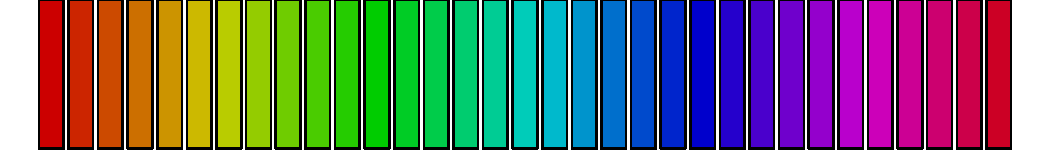
\includegraphics{_main_files/figure-latex/unnamed-chunk-28-1.pdf}

\hypertarget{enunciate-exception-columns}{%
\section{Enunciate exception columns}\label{enunciate-exception-columns}}

Create a vector that enunciate which ordinal variables have ``none'' as a exceptional value when calculating the distance between values.

\begin{Shaded}
\begin{Highlighting}[]
\NormalTok{excep_cols <-}\StringTok{ }\KeywordTok{c}\NormalTok{(}\StringTok{"INCLUS_DISTRIB"}\NormalTok{,}\StringTok{"INCLUS_ORIENT"}\NormalTok{,}\StringTok{"COAR_ROUNDNESS"}\NormalTok{,}
                \StringTok{"COAR_FORM"}\NormalTok{,}\StringTok{"COAR_SPACING"}\NormalTok{,}\StringTok{"COAR_SORTING"}\NormalTok{,}\StringTok{"FINE_FORM"}\NormalTok{)}
\end{Highlighting}
\end{Shaded}

In order to understand this ``exceptional value'' feature, compare the levels of regular and exceptional variables. However, to do that at this point you must re-assure the order of petrographic variables (i.e.~format factors levels):

\begin{Shaded}
\begin{Highlighting}[]
\NormalTok{cleanAmphorae <-}\StringTok{ }\KeywordTok{order_petro}\NormalTok{(cleanAmphorae)}
\end{Highlighting}
\end{Shaded}

This step is not necessary for applying the protocols because the apply\_ordination function already does it internally, before calculating distances.

\begin{longtable}[]{@{}cc@{}}
\toprule
\begin{minipage}[b]{0.22\columnwidth}\centering
Variable\strut
\end{minipage} & \begin{minipage}[b]{0.43\columnwidth}\centering
Values\strut
\end{minipage}\tabularnewline
\midrule
\endhead
\begin{minipage}[t]{0.22\columnwidth}\centering
INCLUS\_DISTRIB\strut
\end{minipage} & \begin{minipage}[t]{0.43\columnwidth}\centering
poorly, poorly to moderately,
moderately, moderately to
well, well, none\strut
\end{minipage}\tabularnewline
\begin{minipage}[t]{0.22\columnwidth}\centering
TEMP\strut
\end{minipage} & \begin{minipage}[t]{0.43\columnwidth}\centering
unfired, 700-800oC, 800-900oC,
900-1000oC, 1000-1100oC\strut
\end{minipage}\tabularnewline
\begin{minipage}[t]{0.22\columnwidth}\centering
COAR\_FREQ\strut
\end{minipage} & \begin{minipage}[t]{0.43\columnwidth}\centering
none, very few, few, common,
abundant, very abundant\strut
\end{minipage}\tabularnewline
\begin{minipage}[t]{0.22\columnwidth}\centering
COAR\_ROUNDNESS\strut
\end{minipage} & \begin{minipage}[t]{0.43\columnwidth}\centering
angular, angular to
subangular, subangular,
subangular to subrounded,
subrounded, subrounded to
rounded, rounded, none\strut
\end{minipage}\tabularnewline
\begin{minipage}[t]{0.22\columnwidth}\centering
COAR\_R\_CALS\strut
\end{minipage} & \begin{minipage}[t]{0.43\columnwidth}\centering
none, few, common, frequent,
dominant, predominant\strut
\end{minipage}\tabularnewline
\begin{minipage}[t]{0.22\columnwidth}\centering
FINE\_FORM\strut
\end{minipage} & \begin{minipage}[t]{0.43\columnwidth}\centering
elongate, elongate to
equidimensional,
equidimensional,
equidimensional to laminar,
laminar, none\strut
\end{minipage}\tabularnewline
\begin{minipage}[t]{0.22\columnwidth}\centering
FINE\_C\_QTZ\strut
\end{minipage} & \begin{minipage}[t]{0.43\columnwidth}\centering
none, few, frequent,
predominant\strut
\end{minipage}\tabularnewline
\bottomrule
\end{longtable}

\hypertarget{choose-geochemical-data}{%
\section{Choose geochemical data}\label{choose-geochemical-data}}

\begin{Shaded}
\begin{Highlighting}[]
\NormalTok{chemVars16 <-}\StringTok{ }\KeywordTok{c}\NormalTok{(}\StringTok{"Fe2O3"}\NormalTok{,}\StringTok{"Al2O3"}\NormalTok{,}\StringTok{"TiO2"}\NormalTok{,}\StringTok{"MgO"}\NormalTok{,}\StringTok{"CaO"}\NormalTok{,}\StringTok{"SiO2"}\NormalTok{,}
                \StringTok{"Th"}\NormalTok{,}\StringTok{"Nb"}\NormalTok{,}\StringTok{"Zr"}\NormalTok{,}\StringTok{"Y"}\NormalTok{,}\StringTok{"Ce"}\NormalTok{,}\StringTok{"Ga"}\NormalTok{,}\StringTok{"V"}\NormalTok{,}\StringTok{"Zn"}\NormalTok{,}\StringTok{"Ni"}\NormalTok{,}\StringTok{"Cr"}\NormalTok{)}
\end{Highlighting}
\end{Shaded}

\hypertarget{save-transformed-geochemical-data-to-file-optional}{%
\section{Save transformed geochemical data to file (optional)}\label{save-transformed-geochemical-data-to-file-optional}}

There is no need to save it in the environment, because \textbf{apply\_ordination} will transform
the data internally and save the results in ``ordination\_object\$transformed\_data'',
when applicable.

\begin{Shaded}
\begin{Highlighting}[]
\KeywordTok{write}\NormalTok{(}\KeywordTok{transform_coda}\NormalTok{(cleanAmphorae,}
                     \DataTypeTok{coda_variables =}\NormalTok{ chemVars16,}
                     \DataTypeTok{method =} \KeywordTok{c}\NormalTok{(}\StringTok{"CLR"}\NormalTok{)),}
      \DataTypeTok{file =} \KeywordTok{paste}\NormalTok{(directories}\OperatorTok{$}\NormalTok{transCoDa, }
                   \StringTok{"transAmphorae_clr.csv"}\NormalTok{, }
                   \DataTypeTok{sep =} \StringTok{"/"}\NormalTok{))}
\end{Highlighting}
\end{Shaded}

In the output table, columns will be ordered as:

\begin{enumerate}
\def\labelenumi{\arabic{enumi}.}
\tightlist
\item
  variables not transformed,
\item
  Raw version of the selected variables,
\item
  Transformed version of the selected variables.
\end{enumerate}

\hypertarget{other-coda-packages}{%
\section{Other CoDa packages}\label{other-coda-packages}}

Be aware that compositional data (CoDa) analysis can be much more complex than what cerUB currently allows for. For more possibilities, you may explore other R packages: \href{https://cran.r-project.org/web/packages/compositions/index.html}{\emph{compositions}}, \href{https://cran.r-project.org/web/packages/zCompositions/index.html}{\emph{zCompositions}}, and \href{https://cran.r-project.org/web/packages/robCompositions/index.html}{\emph{robCompositions}}.

However, before jumping into using more complex techniques, we do recommend a deeper introduction
to CoDa:

\begin{quote}
Pawlowsky-Glahn, V., Buccianti, A., 2011. Compositional data analysis: theory and applications. Wiley.
\end{quote}

\hypertarget{prot1}{%
\chapter{Protocol 1 - Geochemical data}\label{prot1}}

The following example applies protocol 1 to confirm the workshops' chemical reference groups.

Protocol 1 consist in:

\begin{enumerate}
\def\labelenumi{\arabic{enumi}.}
\tightlist
\item
  Select \textbf{\emph{geochemical}} compositional data (CoDa);
\item
  Apply \textbf{\emph{transformation}};
\item
  Perform \textbf{\emph{robust Principal Components Analysis}} (robPCA), implicitly using Euclidean distance;
\item
  Perform \textbf{\emph{PERMANOVA \& PERMDISP}} tests;
\end{enumerate}

Last, search for outliers and re-do protocol excluding outliers.

NOTE: The \protect\hyperlink{init}{initial procedures} must be ran at least once before any protocol can be applied.

\hypertarget{ordination-procedure}{%
\section{Ordination procedure}\label{ordination-procedure}}

\begin{Shaded}
\begin{Highlighting}[]
\NormalTok{prot1 <-}\StringTok{ }\KeywordTok{apply_ordination}\NormalTok{(cleanAmphorae[}\OperatorTok{!}\NormalTok{isShipwreck,], }\CommentTok{# no shipwrecks}
                          \StringTok{"1"}\NormalTok{, }\CommentTok{# select protocol 1}
                          \DataTypeTok{coda_override =}\NormalTok{ chemVars16,}
                          \DataTypeTok{coda_transformation_method =} \StringTok{"ILR"}\NormalTok{)}
\CommentTok{#> [1] "78.24% of variance explained in 2D"}
\CommentTok{#> [1] "86.54% of variance explained in 3D"}
\CommentTok{#> [1] "Protocol 1 ended."}
\end{Highlighting}
\end{Shaded}

The outcome is an \emph{ordination object}. In this case, it is the output of \textbf{pcaCoDa} function in \emph{robCompositions} package, in addition to several extra information, such as the transformed data (`transformed\_data'), the distance matrix (`dist\_matrix'), and the ready-to-plot texts indicating the fitness of the 2D/3D projections respect the distance matrix (`sub2d', `sub3d'). The later are printed in the console once the object is created.

\begin{Shaded}
\begin{Highlighting}[]
\KeywordTok{class}\NormalTok{(prot1)}
\CommentTok{#> [1] "pcaCoDa"}

\KeywordTok{names}\NormalTok{(prot1)}
\CommentTok{#>  [1] "scores"                "loadings"             }
\CommentTok{#>  [3] "eigenvalues"           "method"               }
\CommentTok{#>  [5] "princompOutputClr"     "mult_comp"            }
\CommentTok{#>  [7] "seed"                  "init_seed"            }
\CommentTok{#>  [9] "samples"               "sub2D"                }
\CommentTok{#> [11] "sub3D"                 "transformation_method"}
\CommentTok{#> [13] "transformed_data"      "dist_matrix"          }
\CommentTok{#> [15] "name"}
\end{Highlighting}
\end{Shaded}

\hypertarget{simplify-coda-names}{%
\section{Simplify CoDa names}\label{simplify-coda-names}}

We may want to simplify the names of the transformed variables before plotting them in a biplot. The \textbf{transform\_coda} function, which is called inside \textbf{apply\_ordination} for protocol 1, generates composite names with format ``transformationMethod-component'' for all transformed variables (e.g., ``CLR-Fe2O3''). The \textbf{simplify\_coda\_names} function replaces these names back to the shorter version (e.g., ``Fe2O3''). However, you must always remember that the variables projected in biplots are not the originals but the transformed versions. This is particularly important when dealing with log-ratio variables since they contain information that goes beyond the original variable (i.e., divider).

\begin{Shaded}
\begin{Highlighting}[]
\NormalTok{prot1 <-}\StringTok{ }\KeywordTok{simplify_coda_names}\NormalTok{(prot1)}
\end{Highlighting}
\end{Shaded}

\hypertarget{test-the-given-chemical-reference-groups}{%
\section{Test the given chemical reference groups}\label{test-the-given-chemical-reference-groups}}

Perform four tests (\textbf{anosim}, \textbf{betadisper}, \textbf{permdisp2}, and \textbf{permanova}) that assess the separation and uniformity of the given group factor. For more details on these tests, we refer to:

\begin{quote}
Anderson, M.J., Walsh, D.C.I., 2013. PERMANOVA, ANOSIM, and the Mantel test in the face of heterogeneous dispersions: What null hypothesis are you testing? Ecol. Monogr. 83, 557-574. \url{doi:10.1890/12-2010.1}
\end{quote}

The whole test batch may take several minutes depending on the size of the data matrix and the number of groups.

\begin{Shaded}
\begin{Highlighting}[]
\NormalTok{prot1_tests <-}\StringTok{ }\KeywordTok{test_groups}\NormalTok{(prot1}\OperatorTok{$}\NormalTok{dist_matrix, factor_list}\OperatorTok{$}\NormalTok{ChemGroup)}
\CommentTok{#> [1] "initiating test batch..."}
\CommentTok{#> [1] "vegan::anosim done."}
\CommentTok{#> [1] "vegan::betadisper done."}
\CommentTok{#> [1] "vegan::permutest done."}
\CommentTok{#> [1] "vegan::adonis done."}
\CommentTok{#> [1] "Test batch completed."}
\end{Highlighting}
\end{Shaded}

The tests outputs can be accessed by their name:

\begin{Shaded}
\begin{Highlighting}[]
\KeywordTok{names}\NormalTok{(prot1_tests)}
\CommentTok{#> [1] "permanova" "betadisp"  "permdisp2" "anosim"    "text"}
\end{Highlighting}
\end{Shaded}

The object also contains a ``text'' object, which is a function that generates a list of text lines for plotting the results of PERMANOVA and PERMDISP2 tests. It may feel confusing, but keep in mind that this ``portable'' function requires the same ordination object as an argument.

\begin{Shaded}
\begin{Highlighting}[]
\NormalTok{displayTestText <-}\StringTok{ }\ControlFlowTok{function}\NormalTok{(test_text) \{}
  \KeywordTok{par}\NormalTok{(}\DataTypeTok{mar =} \KeywordTok{c}\NormalTok{(}\DecValTok{0}\NormalTok{, }\DecValTok{0}\NormalTok{, }\DecValTok{0}\NormalTok{, }\DecValTok{0}\NormalTok{), }\DataTypeTok{fig =} \KeywordTok{c}\NormalTok{(}\FloatTok{0.05}\NormalTok{, }\FloatTok{0.9}\NormalTok{, }\FloatTok{0.05}\NormalTok{, }\FloatTok{0.9}\NormalTok{))}
  \KeywordTok{plot.new}\NormalTok{()}
  \ControlFlowTok{for}\NormalTok{ (i }\ControlFlowTok{in} \DecValTok{1}\OperatorTok{:}\KeywordTok{length}\NormalTok{(test_text)) \{}
    
    \CommentTok{# this is for calculating the vertical }
    \CommentTok{# position of paragraphs and lines}
\NormalTok{    test_spacing_paragraph =}\StringTok{ }\FloatTok{0.8}
\NormalTok{    test_spacing_line =}\StringTok{ }\FloatTok{0.8}
    
\NormalTok{    first_line_pos_y <-}
\StringTok{      }\DecValTok{1} \OperatorTok{-}\StringTok{ }\NormalTok{test_spacing_paragraph }\OperatorTok{*}\StringTok{ }\NormalTok{( (i }\OperatorTok{-}\StringTok{ }\FloatTok{.9}\NormalTok{) }\OperatorTok{/}\StringTok{ }\KeywordTok{length}\NormalTok{(test_text) )}
    
\NormalTok{    pos_y <-}\StringTok{ }\NormalTok{first_line_pos_y}
    
    \ControlFlowTok{if}\NormalTok{ (}\KeywordTok{length}\NormalTok{(test_text[[i]]) }\OperatorTok{>}\StringTok{ }\DecValTok{1}\NormalTok{) \{}
      
\NormalTok{      next_paragraph_pos_y <-}
\StringTok{        }\DecValTok{1} \OperatorTok{-}\StringTok{ }\NormalTok{test_spacing_paragraph }\OperatorTok{*}\StringTok{ }\NormalTok{( i }\OperatorTok{/}\StringTok{ }\KeywordTok{length}\NormalTok{(test_text) )}
      
      \ControlFlowTok{for}\NormalTok{ (j }\ControlFlowTok{in} \DecValTok{2}\OperatorTok{:}\KeywordTok{length}\NormalTok{((test_text[[i]])))}
\NormalTok{      \{}
\NormalTok{        pos_y <-}
\StringTok{          }\KeywordTok{c}\NormalTok{(pos_y,}
\NormalTok{            first_line_pos_y }\OperatorTok{-}\StringTok{ }\NormalTok{test_spacing_line }\OperatorTok{*}\StringTok{ }
\StringTok{              }\NormalTok{((j }\OperatorTok{-}\StringTok{ }\DecValTok{1}\NormalTok{) }\OperatorTok{/}\StringTok{ }\NormalTok{(}\KeywordTok{length}\NormalTok{((test_text[[i]])))) }\OperatorTok{*}\StringTok{ }
\StringTok{              }\NormalTok{(first_line_pos_y }\OperatorTok{-}\StringTok{ }\NormalTok{next_paragraph_pos_y)}
\NormalTok{          )}
\NormalTok{      \}}
\NormalTok{    \}}
    \CommentTok{# display a paragraph (a element of the list)}
    \KeywordTok{text}\NormalTok{(}\DecValTok{0}\NormalTok{, pos_y, }\DataTypeTok{labels =}\NormalTok{ test_text[[i]], }\DataTypeTok{cex =} \FloatTok{0.8}\NormalTok{, }\DataTypeTok{pos =} \DecValTok{4}\NormalTok{)}
\NormalTok{  \}}
\NormalTok{\}}

\KeywordTok{displayTestText}\NormalTok{(prot1_tests}\OperatorTok{$}\KeywordTok{text}\NormalTok{(prot1_tests))}
\end{Highlighting}
\end{Shaded}

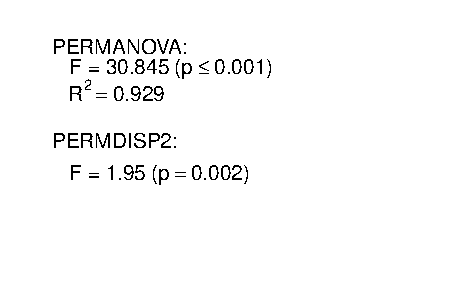
\includegraphics{_main_files/figure-latex/unnamed-chunk-41-1.pdf}

A rule-of-thumb for interpreting PERMANOVA and PERMDISP2 results is: if both p-values are low enough (e.g.~\textless{} 0.05), the classification given is a good approximation of the data.

\pagebreak

\hypertarget{biplot}{%
\section{Biplots}\label{biplot}}

Ordination objects are best represented in biplots, which simultaneously display the projections of observations (points) and variables (arrows) over the same space. There are several options for creating biplots in R, starting with the readily available \textbf{biplot} function:

\begin{Shaded}
\begin{Highlighting}[]
\KeywordTok{biplot}\NormalTok{(prot1)}
\end{Highlighting}
\end{Shaded}

\begin{figure}
\centering
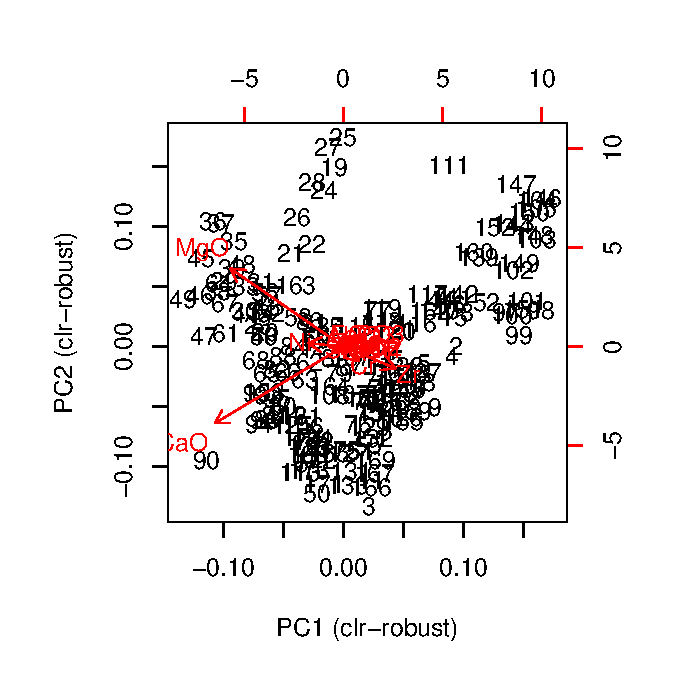
\includegraphics{_main_files/figure-latex/unnamed-chunk-42-1.pdf}
\caption{\label{fig:unnamed-chunk-42}Default biplot in R}
\end{figure}

Although there are several options for customizing this default biplot function, we recommend the use of the \emph{biplot2d3d} package. This package wraps a lot of possibilities in R.

\begin{Shaded}
\begin{Highlighting}[]
\KeywordTok{library}\NormalTok{(biplot2d3d)}
\end{Highlighting}
\end{Shaded}

The \emph{biplot2d3d} package use functions of other packages to allow the customization of virtually all aspects of a biplot. Another important feature of this package is the creation of three-dimensional interactive biplots using the \emph{rgl} package.

\pagebreak

\hypertarget{biplot-2d}{%
\subsection{Biplot 2D}\label{biplot-2d}}

You can consult all tuning options available in the \textbf{biplot\_2d} function by calling up the help file:

\begin{Shaded}
\begin{Highlighting}[]
\NormalTok{?biplot_2d}
\end{Highlighting}
\end{Shaded}

The default configuration will probably give you a much clearer picture than the \textbf{biplot} function, specially if your dataset contains more than 100 observations.

\begin{Shaded}
\begin{Highlighting}[]
\KeywordTok{biplot_2d}\NormalTok{(prot1)}
\end{Highlighting}
\end{Shaded}

\begin{figure}
\centering
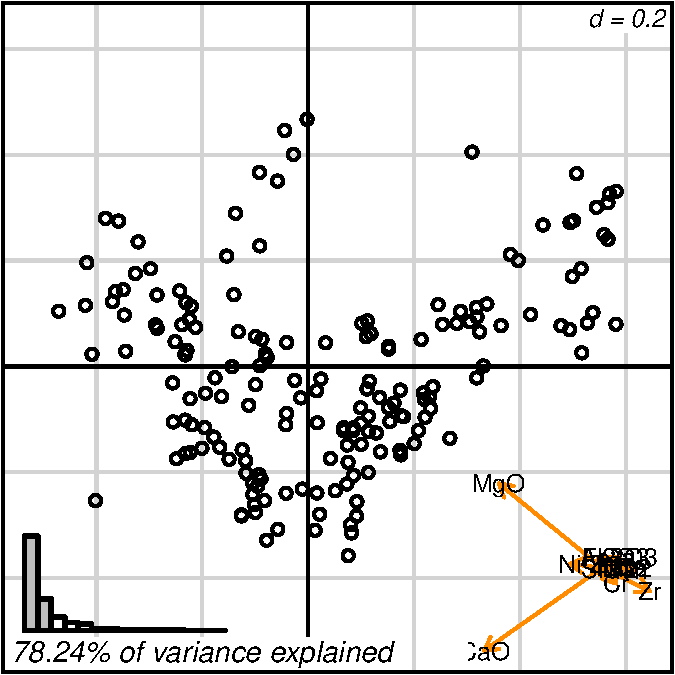
\includegraphics{_main_files/figure-latex/unnamed-chunk-46-1.pdf}
\caption{\label{fig:unnamed-chunk-46}default 2D}
\end{figure}

\pagebreak

The default setting detaches the variables projections (arrows) and places them as a miniature in the bottom-right corner. In this format they may still be interpreted, much like the North when reading a map. Remember though: the more longer arrows you see, the less each one of them is reliable when comparing point values. Here, we were `lucky' for getting two nearly orthogonal variables (CaO and MgO), which means, for instance, that those observations in the bottom-left corner are surely more calcareous than those in the top-right. See the \href{8_Appendix_biplot.html}{Appendix section} for more details.

If detaching the arrows is not of your preference, you can disable this:

\begin{Shaded}
\begin{Highlighting}[]
\KeywordTok{biplot_2d}\NormalTok{(prot1, }
          \DataTypeTok{detach_arrows =} \OtherTok{FALSE}\NormalTok{, }
          \DataTypeTok{output_type =} \StringTok{"preview"}\NormalTok{)}
\end{Highlighting}
\end{Shaded}

\begin{figure}
\centering
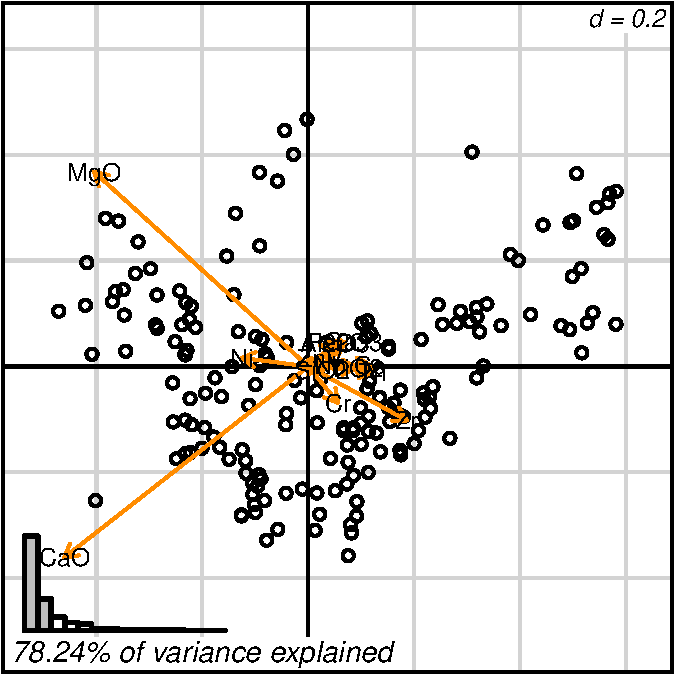
\includegraphics{_main_files/figure-latex/unnamed-chunk-47-1.pdf}
\caption{\label{fig:unnamed-chunk-47}detach\_arrows = FALSE}
\end{figure}

\pagebreak

You can also visualize how the projection of points respond to a given typology (in this case, the chemical reference groups defined in previous studies).

\begin{Shaded}
\begin{Highlighting}[]
\KeywordTok{biplot_2d}\NormalTok{(prot1, }
          \DataTypeTok{groups =}\NormalTok{ factor_list}\OperatorTok{$}\NormalTok{ChemGroup,}
          \DataTypeTok{output_type =} \StringTok{"preview"}\NormalTok{)}
\end{Highlighting}
\end{Shaded}

\begin{figure}
\centering
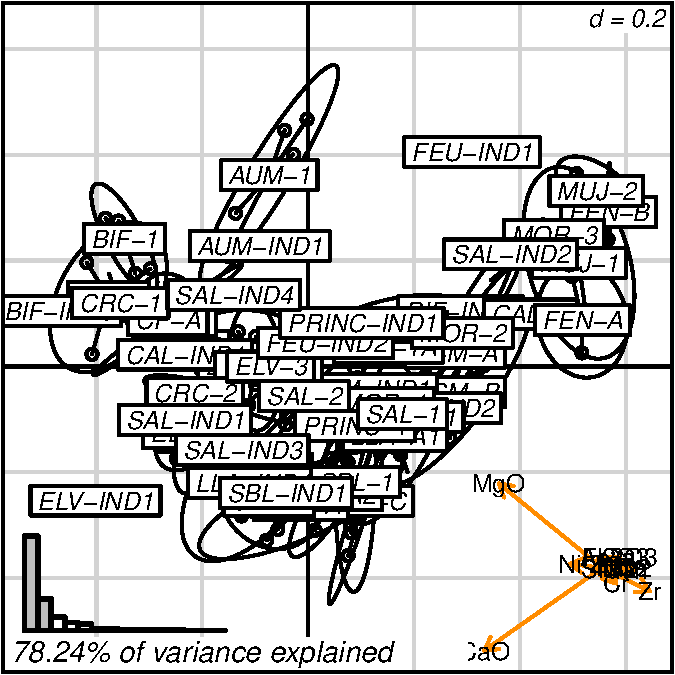
\includegraphics{_main_files/figure-latex/unnamed-chunk-48-1.pdf}
\caption{\label{fig:unnamed-chunk-48}default with groups}
\end{figure}

\pagebreak

To get a prettier plot or match your research needs, you can play with the options given by the \textbf{biplot\_2d}.\\
Note that groups are by default marked using inertia ellipses. They can only be interpreted as confidence ellipses if each group can be assumed to be normally distributed in all variables considered (see more details on the scaling factor ``group\_ellipse\_cex'' in the help file). This is often not reasonable concerning groups that are either too small (\textless{} 10) or contain subgroups.\\
In the argument ``test\_text'' you can introduce the ``text'' function of the ``prot1\_tests'' object.

\begin{Shaded}
\begin{Highlighting}[]
\KeywordTok{biplot_2d}\NormalTok{(prot1, }
          \DataTypeTok{groups =}\NormalTok{ factor_list}\OperatorTok{$}\NormalTok{ChemGroup, }
          \DataTypeTok{group_color =}\NormalTok{ color_list}\OperatorTok{$}\NormalTok{ChemGroup,}
          \DataTypeTok{group_label_cex =} \FloatTok{0.6}\NormalTok{,}
          \DataTypeTok{invert_coordinates =} \KeywordTok{c}\NormalTok{(}\OtherTok{TRUE}\NormalTok{, }\OtherTok{TRUE}\NormalTok{),}
          \DataTypeTok{arrow_label_cex =} \FloatTok{0.7}\NormalTok{,}
          \DataTypeTok{test_text =}\NormalTok{ prot1_tests}\OperatorTok{$}\KeywordTok{text}\NormalTok{(prot1_tests),}
          \DataTypeTok{test_cex =} \FloatTok{0.8}\NormalTok{,}
          \DataTypeTok{test_fig =} \KeywordTok{c}\NormalTok{(}\DecValTok{0}\NormalTok{, }\FloatTok{0.5}\NormalTok{, }\FloatTok{0.65}\NormalTok{, }\FloatTok{.99}\NormalTok{),}
          \DataTypeTok{output_type =} \StringTok{"preview"}\NormalTok{)}
\end{Highlighting}
\end{Shaded}

\begin{figure}
\centering
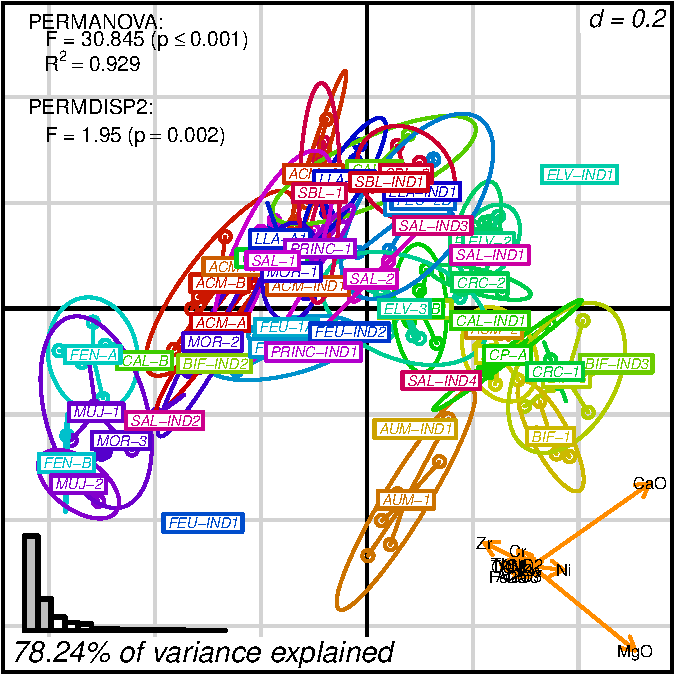
\includegraphics{_main_files/figure-latex/unnamed-chunk-49-1.pdf}
\caption{\label{fig:unnamed-chunk-49}tunning appearance, groups with colors}
\end{figure}

\pagebreak

\begin{Shaded}
\begin{Highlighting}[]
\KeywordTok{biplot_2d}\NormalTok{(prot1, }
          \DataTypeTok{groups =}\NormalTok{ factor_list}\OperatorTok{$}\NormalTok{ChemGroup, }
          \DataTypeTok{group_color =}\NormalTok{ color_list}\OperatorTok{$}\NormalTok{ChemGroup,}
          \DataTypeTok{group_label_cex =} \DecValTok{0}\NormalTok{,}
          \DataTypeTok{group_star_cex =} \DecValTok{0}\NormalTok{,}
          \DataTypeTok{group_ellipse_cex =} \DecValTok{0}\NormalTok{,}
          \DataTypeTok{point_type =} \StringTok{"label"}\NormalTok{,}
          \DataTypeTok{point_label =} \KeywordTok{row.names}\NormalTok{(cleanAmphorae)[}\OperatorTok{!}\NormalTok{isShipwreck],}
          \DataTypeTok{point_label_cex =} \FloatTok{0.5}\NormalTok{,}
          \DataTypeTok{invert_coordinates =} \KeywordTok{c}\NormalTok{(}\OtherTok{TRUE}\NormalTok{, }\OtherTok{TRUE}\NormalTok{),}
          \DataTypeTok{arrow_label_cex =} \FloatTok{0.7}\NormalTok{,}
          \DataTypeTok{test_text =}\NormalTok{ prot1_tests}\OperatorTok{$}\KeywordTok{text}\NormalTok{(prot1_tests),}
          \DataTypeTok{test_cex =} \FloatTok{0.8}\NormalTok{,}
          \DataTypeTok{test_fig =} \KeywordTok{c}\NormalTok{(}\DecValTok{0}\NormalTok{, }\FloatTok{0.5}\NormalTok{, }\FloatTok{0.65}\NormalTok{, }\FloatTok{.99}\NormalTok{),}
          \DataTypeTok{output_type =} \StringTok{"preview"}\NormalTok{)}
\end{Highlighting}
\end{Shaded}

\begin{figure}
\centering
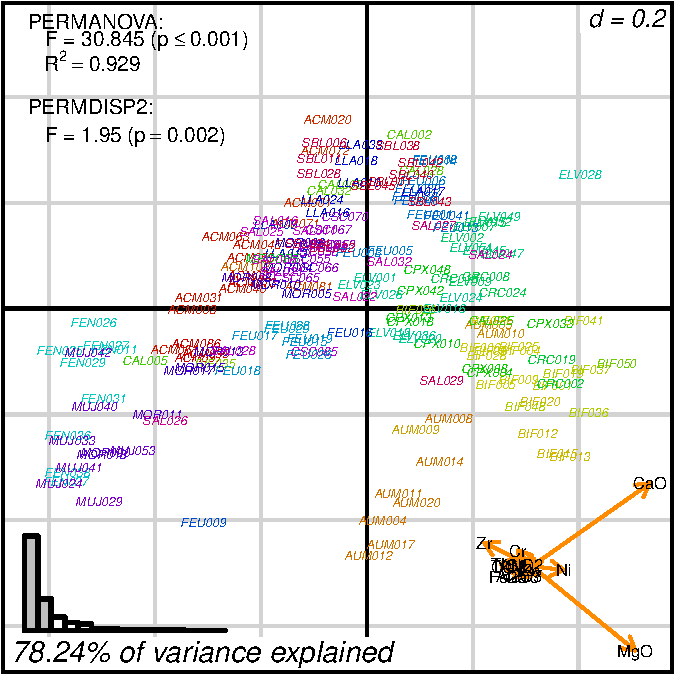
\includegraphics{_main_files/figure-latex/unnamed-chunk-50-1.pdf}
\caption{\label{fig:unnamed-chunk-50}labeled points}
\end{figure}

\pagebreak

It is also possible to save 2D biplots into various file formats (png, tiff, jpeg, eps):

\begin{Shaded}
\begin{Highlighting}[]
\CommentTok{# better PNG version}
\KeywordTok{biplot_2d}\NormalTok{(prot1,}
          \DataTypeTok{ordination_method =} \StringTok{"PCA"}\NormalTok{,}
          \DataTypeTok{invert_coordinates =} \KeywordTok{c}\NormalTok{ (}\OtherTok{TRUE}\NormalTok{,}\OtherTok{TRUE}\NormalTok{),}
          \DataTypeTok{grid_cex =} \FloatTok{2.5}\NormalTok{,}
          \DataTypeTok{ylim =} \KeywordTok{c}\NormalTok{(}\OperatorTok{-}\NormalTok{.}\DecValTok{1}\NormalTok{,.}\DecValTok{1}\NormalTok{),}
          \DataTypeTok{point_type =} \StringTok{"point"}\NormalTok{,}
          \DataTypeTok{groups =}\NormalTok{ factor_list}\OperatorTok{$}\NormalTok{ChemGroup,}
          \DataTypeTok{group_color =}\NormalTok{ color_list}\OperatorTok{$}\NormalTok{ChemGroup,}
          \DataTypeTok{group_label_cex =} \FloatTok{1.5}\NormalTok{,}
          \DataTypeTok{arrow_label_cex =} \DecValTok{2}\NormalTok{,}
          \DataTypeTok{arrow_cex =} \FloatTok{0.2}\NormalTok{,}
          \DataTypeTok{arrow_lwd =} \FloatTok{2.5}\NormalTok{,}
          \DataTypeTok{arrow_fig =} \KeywordTok{c}\NormalTok{(.}\DecValTok{6}\NormalTok{,.}\DecValTok{95}\NormalTok{,}\DecValTok{0}\NormalTok{,.}\DecValTok{35}\NormalTok{),}
          \DataTypeTok{subtitle_cex =} \FloatTok{2.5}\NormalTok{,}
          \DataTypeTok{test_text =}\NormalTok{ prot1_tests}\OperatorTok{$}\KeywordTok{text}\NormalTok{(prot1_tests),}
          \DataTypeTok{test_fig =}\KeywordTok{c}\NormalTok{(}\DecValTok{0}\NormalTok{, }\FloatTok{0.5}\NormalTok{, }\FloatTok{0.62}\NormalTok{, }\FloatTok{.99}\NormalTok{),}
          \DataTypeTok{test_cex =} \DecValTok{2}\NormalTok{,}
          \DataTypeTok{fitAnalysis_fig =} \KeywordTok{c}\NormalTok{(}\DecValTok{0}\NormalTok{,.}\DecValTok{7}\NormalTok{,.}\DecValTok{05}\NormalTok{,.}\DecValTok{5}\NormalTok{),}
          \CommentTok{# saving settings}
          \DataTypeTok{file_name =} \StringTok{"Prot1_Biplot2D"}\NormalTok{,}
          \DataTypeTok{directory =}\NormalTok{ directories}\OperatorTok{$}\NormalTok{prot1,}
          \DataTypeTok{width =} \DecValTok{1000}\NormalTok{, }\DataTypeTok{height =} \DecValTok{1000}\NormalTok{,}
          \DataTypeTok{output_type =} \StringTok{"png"}\NormalTok{)}
\end{Highlighting}
\end{Shaded}

\pagebreak

\hypertarget{biplot-3d}{%
\subsection{Biplot 3D}\label{biplot-3d}}

Most 2D options are also available when generating 3D biplots. Consult the help file for details.

\begin{Shaded}
\begin{Highlighting}[]
\NormalTok{?biplot_3d}
\end{Highlighting}
\end{Shaded}

\begin{Shaded}
\begin{Highlighting}[]
\KeywordTok{biplot_3d}\NormalTok{(prot1,}
          \DataTypeTok{ordination_method =} \StringTok{"PCA"}\NormalTok{,}
          \DataTypeTok{groups =}\NormalTok{ factor_list}\OperatorTok{$}\NormalTok{ChemGroup,}
          \DataTypeTok{group_color =}\NormalTok{ color_list}\OperatorTok{$}\NormalTok{ChemGroup,}
          \DataTypeTok{point_type =} \StringTok{"point"}\NormalTok{,}
          \DataTypeTok{group_representation =} \StringTok{"stars"}\NormalTok{,}
          \DataTypeTok{star_centroid_radius =} \DecValTok{0}\NormalTok{,}
          \DataTypeTok{star_label_cex =} \FloatTok{.8}\NormalTok{,}
          \DataTypeTok{test_text =}\NormalTok{ prot1_tests}\OperatorTok{$}\KeywordTok{text}\NormalTok{(prot1_tests),}
          \DataTypeTok{test_cex =} \FloatTok{1.25}\NormalTok{,}
          \DataTypeTok{test_fig =} \KeywordTok{c}\NormalTok{(}\DecValTok{0}\NormalTok{, }\FloatTok{0.5}\NormalTok{, }\FloatTok{0.65}\NormalTok{, }\FloatTok{.99}\NormalTok{))}
\end{Highlighting}
\end{Shaded}

\hypertarget{rgl21648}{}

\pagebreak

You can save an animated GIF and a PNG snapshot using the \textbf{animation} function.

\begin{Shaded}
\begin{Highlighting}[]
\NormalTok{biplot2d3d}\OperatorTok{::}\KeywordTok{animation}\NormalTok{(}\DataTypeTok{directory =}\NormalTok{ directories}\OperatorTok{$}\NormalTok{prot1,}
                       \DataTypeTok{file_name =} \StringTok{"Prot1_Biplot3D"}\NormalTok{)}
\end{Highlighting}
\end{Shaded}

You will need to install \href{www.imagemagick.org}{ImageMagick} to be able to generate the GIF animation.

In these images, you get what you would see when running the biplot\_3d function in a regular R session.

NOTE: Animated GIF will not be displayed in the pdf version of this document.

\pagebreak

\hypertarget{comparing-coda-transformations}{%
\section{Comparing CoDa transformations}\label{comparing-coda-transformations}}

There is a lot of debate on which transformation is useful--or even \emph{valid}--for analyzing geochemical compositions in Archaeometry. We show here how you can compare the results of applying different transformations to the same dataset.

First, create different ordination objects for each type of CoDa transformation that you wish to compare:

\begin{Shaded}
\begin{Highlighting}[]
\NormalTok{prot1_std <-}\StringTok{ }\KeywordTok{apply_ordination}\NormalTok{(cleanAmphorae[}\OperatorTok{!}\NormalTok{isShipwreck,],}
                              \StringTok{"1"}\NormalTok{, }\CommentTok{# select protocol 1}
                              \DataTypeTok{coda_override =}\NormalTok{ chemVars16,}
                              \DataTypeTok{coda_transformation =} \StringTok{"std"}\NormalTok{)}
\CommentTok{#> [1] "56.05% of variance explained in 2D"}
\CommentTok{#> [1] "64.91% of variance explained in 3D"}
\CommentTok{#> [1] "Protocol 1 ended."}

\NormalTok{prot1_log <-}\StringTok{ }\KeywordTok{apply_ordination}\NormalTok{(cleanAmphorae[}\OperatorTok{!}\NormalTok{isShipwreck,],}
                              \StringTok{"1"}\NormalTok{, }\CommentTok{# select protocol 1}
                              \DataTypeTok{coda_override =}\NormalTok{ chemVars16,}
                              \DataTypeTok{coda_transformation =} \StringTok{"log"}\NormalTok{)}
\CommentTok{#> [1] "62.66% of variance explained in 2D"}
\CommentTok{#> [1] "72.53% of variance explained in 3D"}
\CommentTok{#> [1] "Protocol 1 ended."}

\NormalTok{prot1_ALR <-}\StringTok{ }\KeywordTok{apply_ordination}\NormalTok{(cleanAmphorae[}\OperatorTok{!}\NormalTok{isShipwreck,],}
                              \StringTok{"1"}\NormalTok{, }\CommentTok{# select protocol 1}
                              \DataTypeTok{coda_override =}\NormalTok{ chemVars16,}
                              \DataTypeTok{coda_transformation =} \StringTok{"ALR"}\NormalTok{,}
                              \CommentTok{# this is the divisor component}
                              \DataTypeTok{coda_alr_base =} \StringTok{"Fe2O3"}\NormalTok{)}
\CommentTok{#> [1] "70.3% of variance explained in 2D"}
\CommentTok{#> [1] "81.75% of variance explained in 3D"}
\CommentTok{#> [1] "Protocol 1 ended."}

\NormalTok{prot1_CLR <-}\StringTok{ }\KeywordTok{apply_ordination}\NormalTok{(cleanAmphorae[}\OperatorTok{!}\NormalTok{isShipwreck,],}
                              \StringTok{"1"}\NormalTok{, }\CommentTok{# select protocol 1}
                              \DataTypeTok{coda_override =}\NormalTok{ chemVars16,}
                              \DataTypeTok{coda_transformation =} \StringTok{"CLR"}\NormalTok{)}
\CommentTok{#> [1] "64.16% of variance explained in 2D"}
\CommentTok{#> [1] "75.57% of variance explained in 3D"}
\CommentTok{#> [1] "Protocol 1 ended."}
\end{Highlighting}
\end{Shaded}

\pagebreak

Then, create the respective biplots:

\begin{Shaded}
\begin{Highlighting}[]
\NormalTok{biplot2d3d}\OperatorTok{::}\KeywordTok{biplot_2d}\NormalTok{(prot1_std,}
                      \DataTypeTok{groups =}\NormalTok{ factor_list}\OperatorTok{$}\NormalTok{ChemGroup,}
                      \DataTypeTok{group_color =}\NormalTok{ color_list}\OperatorTok{$}\NormalTok{ChemGroup,}
                      \DataTypeTok{group_label_cex =} \FloatTok{0.6}\NormalTok{,}
                      \DataTypeTok{arrow_label_cex =} \FloatTok{0.7}\NormalTok{,}
                      \DataTypeTok{ylim =} \KeywordTok{c}\NormalTok{(}\OperatorTok{-}\FloatTok{0.9}\NormalTok{, }\FloatTok{0.6}\NormalTok{),}
                      \DataTypeTok{x_title =} \StringTok{"Scaled and Centred"}\NormalTok{,}
                      \DataTypeTok{x_title_cex =} \FloatTok{1.5}\NormalTok{,}
                      \DataTypeTok{x_title_fig =} \KeywordTok{c}\NormalTok{(}\FloatTok{0.05}\NormalTok{, }\FloatTok{0.9}\NormalTok{, }\FloatTok{0.85}\NormalTok{, }\DecValTok{1}\NormalTok{),}
                      \DataTypeTok{output_type =} \StringTok{"preview"}\NormalTok{)}
\end{Highlighting}
\end{Shaded}

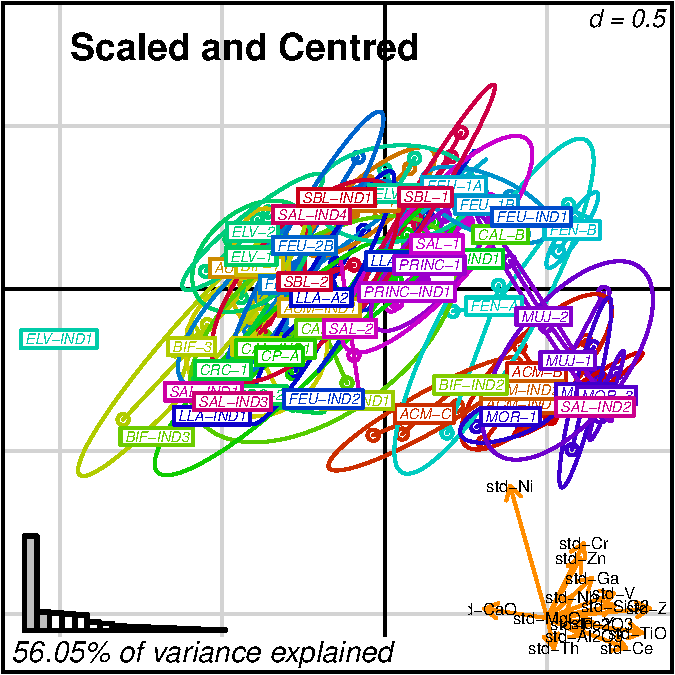
\includegraphics{_main_files/figure-latex/unnamed-chunk-57-1.pdf}

\pagebreak

\begin{Shaded}
\begin{Highlighting}[]
\NormalTok{biplot2d3d}\OperatorTok{::}\KeywordTok{biplot_2d}\NormalTok{(prot1_log,}
                      \DataTypeTok{groups =}\NormalTok{ factor_list}\OperatorTok{$}\NormalTok{ChemGroup,}
                      \DataTypeTok{group_color =}\NormalTok{ color_list}\OperatorTok{$}\NormalTok{ChemGroup,}
                      \DataTypeTok{group_label_cex =} \FloatTok{0.6}\NormalTok{,}
                      \DataTypeTok{arrow_label_cex =} \FloatTok{0.7}\NormalTok{,}
                      \DataTypeTok{ylim =} \KeywordTok{c}\NormalTok{(}\OperatorTok{-}\FloatTok{0.6}\NormalTok{, }\FloatTok{0.6}\NormalTok{),}
                      \DataTypeTok{x_title =} \StringTok{"Log-scaled"}\NormalTok{,}
                      \DataTypeTok{x_title_cex =} \FloatTok{1.5}\NormalTok{,}
                      \DataTypeTok{x_title_fig =} \KeywordTok{c}\NormalTok{(}\FloatTok{0.05}\NormalTok{, }\FloatTok{0.9}\NormalTok{, }\FloatTok{0.85}\NormalTok{, }\DecValTok{1}\NormalTok{),}
                      \DataTypeTok{output_type =} \StringTok{"preview"}\NormalTok{)}
\end{Highlighting}
\end{Shaded}

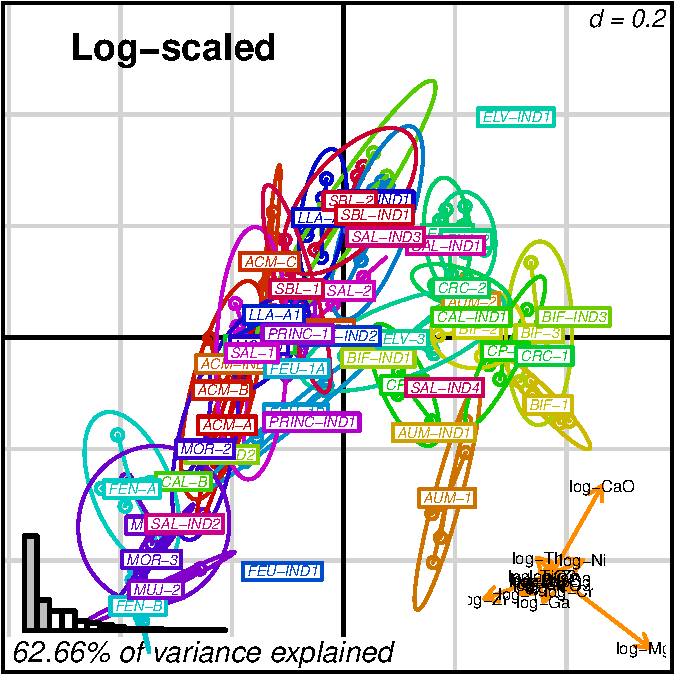
\includegraphics{_main_files/figure-latex/unnamed-chunk-58-1.pdf}

\pagebreak

\begin{Shaded}
\begin{Highlighting}[]
\NormalTok{biplot2d3d}\OperatorTok{::}\KeywordTok{biplot_2d}\NormalTok{(prot1_ALR,}
                      \DataTypeTok{groups =}\NormalTok{ factor_list}\OperatorTok{$}\NormalTok{ChemGroup,}
                      \DataTypeTok{group_color =}\NormalTok{ color_list}\OperatorTok{$}\NormalTok{ChemGroup,}
                      \DataTypeTok{group_label_cex =} \FloatTok{0.6}\NormalTok{,}
                      \DataTypeTok{arrow_label_cex =} \FloatTok{0.7}\NormalTok{,}
                      \DataTypeTok{ylim =} \KeywordTok{c}\NormalTok{(}\OperatorTok{-}\FloatTok{0.6}\NormalTok{, }\FloatTok{0.6}\NormalTok{),}
                      \DataTypeTok{x_title =} \StringTok{"Additive log-ratio"}\NormalTok{,}
                      \DataTypeTok{x_title_cex =} \FloatTok{1.5}\NormalTok{,}
                      \DataTypeTok{x_title_fig =} \KeywordTok{c}\NormalTok{(}\FloatTok{0.05}\NormalTok{, }\FloatTok{0.9}\NormalTok{, }\FloatTok{0.85}\NormalTok{, }\DecValTok{1}\NormalTok{),}
                      \DataTypeTok{output_type =} \StringTok{"preview"}\NormalTok{)}
\end{Highlighting}
\end{Shaded}

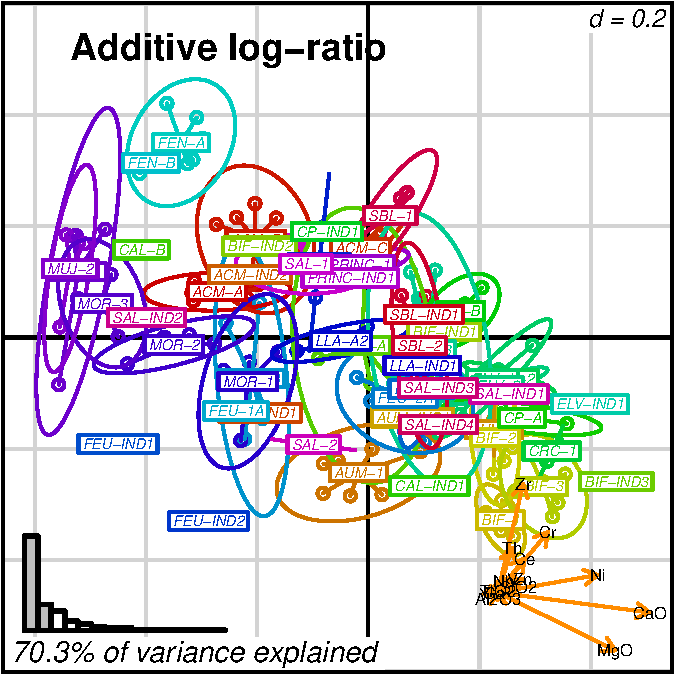
\includegraphics{_main_files/figure-latex/unnamed-chunk-59-1.pdf}

\pagebreak

\begin{Shaded}
\begin{Highlighting}[]
\NormalTok{biplot2d3d}\OperatorTok{::}\KeywordTok{biplot_2d}\NormalTok{(prot1_CLR,}
                      \DataTypeTok{groups =}\NormalTok{ factor_list}\OperatorTok{$}\NormalTok{ChemGroup,}
                      \DataTypeTok{group_color =}\NormalTok{ color_list}\OperatorTok{$}\NormalTok{ChemGroup,}
                      \DataTypeTok{group_label_cex =} \FloatTok{0.6}\NormalTok{,}
                      \DataTypeTok{arrow_label_cex =} \FloatTok{0.7}\NormalTok{,}
                      \DataTypeTok{ylim =} \KeywordTok{c}\NormalTok{(}\OperatorTok{-}\FloatTok{0.5}\NormalTok{, }\FloatTok{0.4}\NormalTok{),}
                      \DataTypeTok{x_title =} \StringTok{"Centred log-ratio"}\NormalTok{,}
                      \DataTypeTok{x_title_cex =} \FloatTok{1.5}\NormalTok{,}
                      \DataTypeTok{x_title_fig =} \KeywordTok{c}\NormalTok{(}\FloatTok{0.05}\NormalTok{, }\FloatTok{0.9}\NormalTok{, }\FloatTok{0.85}\NormalTok{, }\DecValTok{1}\NormalTok{),}
                      \DataTypeTok{output_type =} \StringTok{"preview"}\NormalTok{)}
\end{Highlighting}
\end{Shaded}

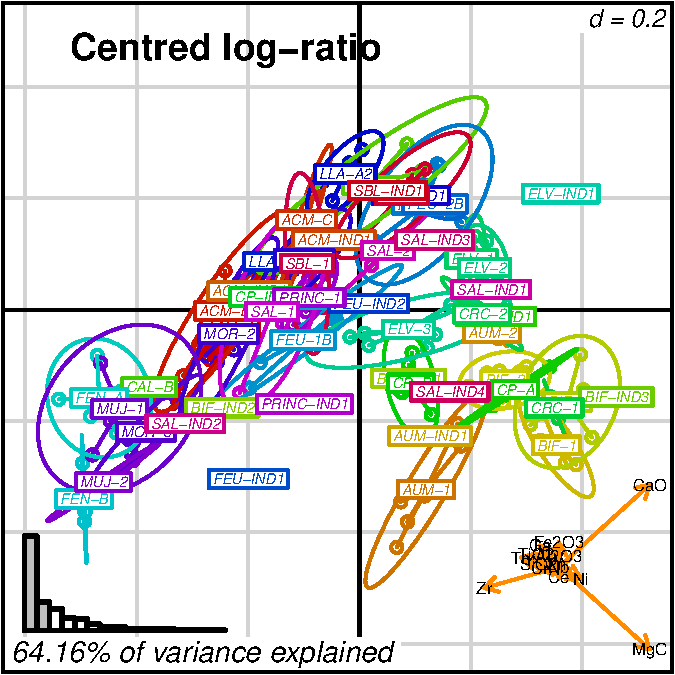
\includegraphics{_main_files/figure-latex/unnamed-chunk-60-1.pdf}

\hypertarget{prot2}{%
\chapter{Protocol 2 - Petrographic data}\label{prot2}}

The following example applies protocol 2 to confirm workshops' petrographic groups.

Protocol 2 consist in:

\begin{enumerate}
\def\labelenumi{\arabic{enumi}.}
\tightlist
\item
  Select ordinal \textbf{\emph{petrographic}} data;
\item
  Transform to \textbf{\emph{ranks}};
\item
  \textbf{\emph{Extended Gower distance}}, using:
\end{enumerate}

\begin{enumerate}
\def\labelenumi{\alph{enumi}.}
\tightlist
\item
  \textbf{Relative ranking difference} (RRD)
\item
  \textbf{Neighbor interchange} (NI)
\end{enumerate}

\begin{enumerate}
\def\labelenumi{\arabic{enumi}.}
\setcounter{enumi}{3}
\tightlist
\item
  Apply ordination procedure:
\end{enumerate}

\begin{enumerate}
\def\labelenumi{\alph{enumi}.}
\tightlist
\item
  \textbf{\emph{Principal Coordinates Analysis}} (PCoA)
\item
  \textbf{\emph{Non-metric Dimensional Scaling}} (NMDS)
\end{enumerate}

\begin{enumerate}
\def\labelenumi{\arabic{enumi}.}
\setcounter{enumi}{4}
\tightlist
\item
  Perform \textbf{\emph{PERMANOVA \& PERMDISP}} tests;
\end{enumerate}

Last, search for outliers and re-do protocol excluding outliers.

NOTE: The \protect\hyperlink{init}{initial procedures} must be ran at least once before any protocol can be applied.

The key references on the Extended Gower distance are:

\begin{quote}
Pavoine, S., Vallet, J., Dufour, A.-B., Gachet, S., Daniel, H., 2009. On the challenge of treating various types of variables: application for improving the measurement of functional diversity. Oikos 118, 391-402. \url{doi:10.1111/j.1600-0706.2008.16668.x}
\end{quote}

\begin{quote}
Podani, J., 1999. Extending Gower's General Coefficient of Similarity to Ordinal Characters on JSTOR. Taxon 48, 331-340. \url{doi:10.2307/1224438}
\end{quote}

\begin{quote}
Gower, J.C., 1971. A General Coefficient of Similarity and Some of Its Properties. Biometrics 27, 857-871. \url{doi:10.2307/2528823}
\end{quote}

\pagebreak

\hypertarget{ordination-procedure-1}{%
\section{Ordination procedure}\label{ordination-procedure-1}}

Depending on which type of distance calculation (RRD/NI), protocol 2 performs different ordination methods (PCoA/NMDS). Both PCoA and NMDS require specifying the number of dimensions in which to project the data. Therefore, you must generate specific 2D and 3D ordination objects:

\begin{Shaded}
\begin{Highlighting}[]
\NormalTok{prot2a_2d <-}\StringTok{ }\KeywordTok{apply_ordination}\NormalTok{(cleanAmphorae[}\OperatorTok{!}\NormalTok{isShipwreck,],}
                              \StringTok{"2a"}\NormalTok{, }\CommentTok{# select protocol 2a (RRD & PCoA)}
                              \DataTypeTok{exception_columns =}\NormalTok{ excep_cols,}
                              \DataTypeTok{variable_tags =}\NormalTok{ varCode)}

\NormalTok{prot2b_2d <-}\StringTok{ }\KeywordTok{apply_ordination}\NormalTok{(cleanAmphorae[}\OperatorTok{!}\NormalTok{isShipwreck,],}
                              \StringTok{"2b"}\NormalTok{, }\CommentTok{# select protocol 2a (NI & NMDS)}
                              \DataTypeTok{exception_columns =}\NormalTok{ excep_cols,}
                              \DataTypeTok{variable_tags =}\NormalTok{ varCode)}

\NormalTok{prot2a_3d <-}\StringTok{ }\KeywordTok{apply_ordination}\NormalTok{(cleanAmphorae[}\OperatorTok{!}\NormalTok{isShipwreck,],}
                              \StringTok{"2a"}\NormalTok{, }\CommentTok{# select protocol 2a (RRD & PCoA)}
                              \DataTypeTok{exception_columns =}\NormalTok{ excep_cols,}
                              \DataTypeTok{variable_tags =}\NormalTok{ varCode,}
                              \DataTypeTok{dimensions =} \DecValTok{3}\NormalTok{)}

\NormalTok{prot2b_3d <-}\StringTok{ }\KeywordTok{apply_ordination}\NormalTok{(cleanAmphorae[}\OperatorTok{!}\NormalTok{isShipwreck,],}
                              \StringTok{"2b"}\NormalTok{, }\CommentTok{# select protocol 2a (NI & NMDS)}
                              \DataTypeTok{exception_columns =}\NormalTok{ excep_cols,}
                              \DataTypeTok{variable_tags =}\NormalTok{ varCode,}
                              \DataTypeTok{dimensions =} \DecValTok{3}\NormalTok{)}
\end{Highlighting}
\end{Shaded}

\pagebreak

The ordination objects generated with protocol 2 are different from those in protocol 1 since it uses different functions. However, the main components are still the same: the projection of observations or \emph{scores} (\textbf{points}) and of variables or \emph{loadings}.

\begin{Shaded}
\begin{Highlighting}[]
\KeywordTok{class}\NormalTok{(prot2a_2d)}
\CommentTok{#> [1] "list"}
\KeywordTok{names}\NormalTok{(prot2a_2d)}
\CommentTok{#>  [1] "points"        "eig"           "x"             "ac"           }
\CommentTok{#>  [5] "GOF"           "sub2D"         "GOF2_2D"       "loadings"     }
\CommentTok{#>  [9] "variable_tags" "name"          "dist_matrix"}
\KeywordTok{class}\NormalTok{(prot2b_2d)}
\CommentTok{#> [1] "metaMDS" "monoMDS"}
\KeywordTok{names}\NormalTok{(prot2b_2d)}
\CommentTok{#>  [1] "nobj"          "nfix"          "ndim"          "ndis"         }
\CommentTok{#>  [5] "ngrp"          "diss"          "iidx"          "jidx"         }
\CommentTok{#>  [9] "xinit"         "istart"        "isform"        "ities"        }
\CommentTok{#> [13] "iregn"         "iscal"         "maxits"        "sratmx"       }
\CommentTok{#> [17] "strmin"        "sfgrmn"        "dist"          "dhat"         }
\CommentTok{#> [21] "points"        "stress"        "grstress"      "iters"        }
\CommentTok{#> [25] "icause"        "call"          "model"         "distmethod"   }
\CommentTok{#> [29] "distcall"      "distance"      "converged"     "tries"        }
\CommentTok{#> [33] "engine"        "species"       "data"          "init_seed"    }
\CommentTok{#> [37] "trymax"        "sub_stress"    "sub2D"         "GOF2_2D"      }
\CommentTok{#> [41] "loadings"      "variable_tags" "name"          "dist_matrix"}
\end{Highlighting}
\end{Shaded}

\pagebreak

\hypertarget{test-the-given-fabric-groups}{%
\section{Test the given fabric groups}\label{test-the-given-fabric-groups}}

The fabric groups defined in previous studies can be tested against Protocol 2 distance matrices. We can use either ``prot2a\_2d\$dist\_matrix'' or ``prot2a\_3d\$dist\_matrix'', because they are the same. Remember that this test batch may take several minutes.

\begin{Shaded}
\begin{Highlighting}[]
\NormalTok{prot2a_tests <-}\StringTok{ }\KeywordTok{test_groups}\NormalTok{(prot2a_2d}\OperatorTok{$}\NormalTok{dist_matrix, }
\NormalTok{                            factor_list}\OperatorTok{$}\NormalTok{FabricGroup)}
\CommentTok{#> [1] "initiating test batch..."}
\CommentTok{#> [1] "vegan::anosim done."}
\CommentTok{#> [1] "vegan::betadisper done."}
\CommentTok{#> [1] "vegan::permutest done."}
\CommentTok{#> [1] "vegan::adonis done."}
\CommentTok{#> [1] "Test batch completed."}
\NormalTok{prot2b_tests <-}\StringTok{ }\KeywordTok{test_groups}\NormalTok{(prot2b_2d}\OperatorTok{$}\NormalTok{dist_matrix,}
\NormalTok{                            factor_list}\OperatorTok{$}\NormalTok{FabricGroup)}
\CommentTok{#> [1] "initiating test batch..."}
\CommentTok{#> [1] "vegan::anosim done."}
\CommentTok{#> Warning in vegan::betadisper(distMatrix, groups): some squared distances}
\CommentTok{#> are negative and changed to zero}
\CommentTok{#> [1] "vegan::betadisper done."}
\CommentTok{#> [1] "vegan::permutest done."}
\CommentTok{#> [1] "vegan::adonis done."}
\CommentTok{#> [1] "Test batch completed."}
\end{Highlighting}
\end{Shaded}

These tests were explained in \protect\hyperlink{tests}{protocol 1}.

\pagebreak

\hypertarget{biplots}{%
\section{Biplots}\label{biplots}}

The details on how to create biplots is already explained in \protect\hyperlink{biplot}{protocol 1}. Concerning protocol 2, we can compare the results of version \emph{2a} (RRD, PCoA) and \emph{2b} (NI, NMDS).

\pagebreak

\hypertarget{biplot-2d-1}{%
\subsection{Biplot 2D}\label{biplot-2d-1}}

\begin{Shaded}
\begin{Highlighting}[]
\NormalTok{arrows_label_adj <-}\StringTok{ }\KeywordTok{rbind}\NormalTok{(}\KeywordTok{c}\NormalTok{(.}\DecValTok{5}\NormalTok{,.}\DecValTok{8}\NormalTok{),}\KeywordTok{c}\NormalTok{(.}\DecValTok{5}\NormalTok{,}\DecValTok{1}\NormalTok{),}\KeywordTok{c}\NormalTok{(.}\DecValTok{5}\NormalTok{,}\DecValTok{1}\NormalTok{),}\KeywordTok{c}\NormalTok{(.}\DecValTok{5}\NormalTok{,}\DecValTok{0}\NormalTok{),}\KeywordTok{c}\NormalTok{(.}\DecValTok{5}\NormalTok{,}\DecValTok{1}\NormalTok{),}
                          \KeywordTok{c}\NormalTok{(.}\DecValTok{5}\NormalTok{,}\DecValTok{0}\NormalTok{),}\KeywordTok{c}\NormalTok{(}\DecValTok{0}\NormalTok{,.}\DecValTok{5}\NormalTok{))}
\KeywordTok{row.names}\NormalTok{(arrows_label_adj) <-}\StringTok{ }\KeywordTok{c}\NormalTok{(}\StringTok{"L48"}\NormalTok{,}\StringTok{"L24"}\NormalTok{,}\StringTok{"L5"}\NormalTok{,}\StringTok{"L36"}\NormalTok{,}\StringTok{"S7"}\NormalTok{,}
                                 \StringTok{"S8"}\NormalTok{,}\StringTok{"S11"}\NormalTok{)}

\NormalTok{biplot2d3d}\OperatorTok{::}\KeywordTok{biplot_2d}\NormalTok{(prot2a_2d,}
                      \DataTypeTok{ordination_method =} \StringTok{"PCoA"}\NormalTok{,}
                      \DataTypeTok{invert_coordinates =} \KeywordTok{c}\NormalTok{ (}\OtherTok{TRUE}\NormalTok{,}\OtherTok{TRUE}\NormalTok{),}
                      \DataTypeTok{xlim =} \KeywordTok{c}\NormalTok{(}\OperatorTok{-}\NormalTok{.}\DecValTok{26}\NormalTok{,.}\DecValTok{35}\NormalTok{),}
                      \DataTypeTok{ylim =} \KeywordTok{c}\NormalTok{(}\OperatorTok{-}\NormalTok{.}\DecValTok{31}\NormalTok{,.}\DecValTok{35}\NormalTok{),}
                      \DataTypeTok{point_type =} \StringTok{"point"}\NormalTok{,}
                      \DataTypeTok{groups =}\NormalTok{ factor_list}\OperatorTok{$}\NormalTok{FabricGroup,}
                      \DataTypeTok{group_color =}\NormalTok{ color_list}\OperatorTok{$}\NormalTok{FabricGroup,}
                      \DataTypeTok{group_label_cex =} \FloatTok{0.6}\NormalTok{,}
                      \DataTypeTok{arrow_mim_dist =} \FloatTok{0.5}\NormalTok{,}
                      \DataTypeTok{arrow_label_cex =} \FloatTok{0.6}\NormalTok{,}
                      \DataTypeTok{arrow_fig =} \KeywordTok{c}\NormalTok{(.}\DecValTok{6}\NormalTok{,.}\DecValTok{95}\NormalTok{,}\DecValTok{0}\NormalTok{,.}\DecValTok{35}\NormalTok{),}
                      \DataTypeTok{arrow_label_adj_override =}\NormalTok{ arrows_label_adj,}
                      \DataTypeTok{subtitle =}\NormalTok{ prot2a_2d}\OperatorTok{$}\NormalTok{sub2D,}
                      \DataTypeTok{test_text =}\NormalTok{ prot2a_tests}\OperatorTok{$}\KeywordTok{text}\NormalTok{(prot2a_tests),}
                      \DataTypeTok{test_cex =} \FloatTok{0.8}\NormalTok{,}
                      \DataTypeTok{test_fig =} \KeywordTok{c}\NormalTok{(}\DecValTok{0}\NormalTok{, }\FloatTok{0.5}\NormalTok{, }\FloatTok{0.62}\NormalTok{, }\FloatTok{.99}\NormalTok{),}
                      \DataTypeTok{fitAnalysis_fig =} \KeywordTok{c}\NormalTok{(}\DecValTok{0}\NormalTok{,.}\DecValTok{7}\NormalTok{,.}\DecValTok{05}\NormalTok{,.}\DecValTok{5}\NormalTok{),}
                      \DataTypeTok{output_type =} \StringTok{"preview"}\NormalTok{)}
\end{Highlighting}
\end{Shaded}

\begin{figure}
\centering
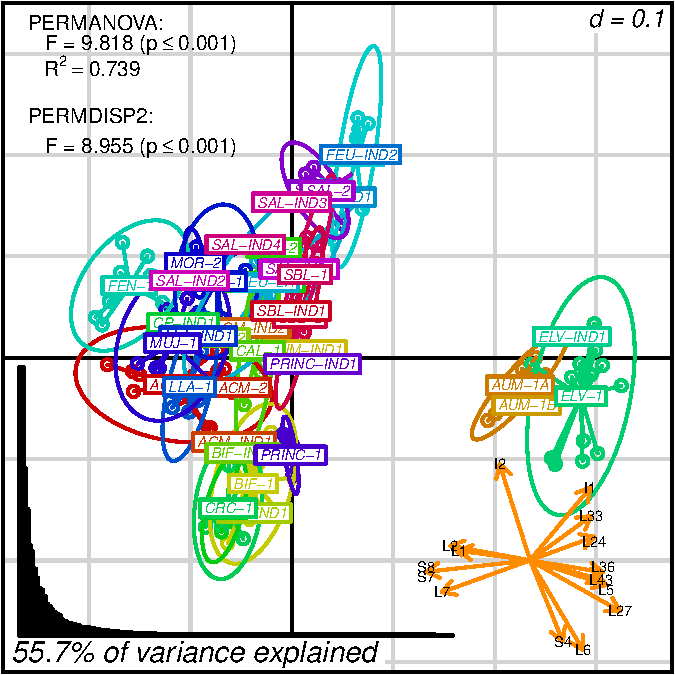
\includegraphics{_main_files/figure-latex/unnamed-chunk-66-1.pdf}
\caption{\label{fig:unnamed-chunk-66}protocol 2a}
\end{figure}

\pagebreak

\begin{Shaded}
\begin{Highlighting}[]
\NormalTok{arrows_label_adj <-}\StringTok{ }\KeywordTok{rbind}\NormalTok{(}\KeywordTok{c}\NormalTok{(.}\DecValTok{5}\NormalTok{,}\DecValTok{1}\NormalTok{),}\KeywordTok{c}\NormalTok{(.}\DecValTok{5}\NormalTok{,}\DecValTok{0}\NormalTok{),}\KeywordTok{c}\NormalTok{(.}\DecValTok{5}\NormalTok{,}\DecValTok{1}\NormalTok{),}\KeywordTok{c}\NormalTok{(.}\DecValTok{5}\NormalTok{,}\DecValTok{1}\NormalTok{),}\KeywordTok{c}\NormalTok{(.}\DecValTok{5}\NormalTok{,}\DecValTok{0}\NormalTok{),}
                          \KeywordTok{c}\NormalTok{(}\DecValTok{0}\NormalTok{,.}\DecValTok{5}\NormalTok{),}\KeywordTok{c}\NormalTok{(}\DecValTok{1}\NormalTok{,.}\DecValTok{5}\NormalTok{))}
\KeywordTok{row.names}\NormalTok{(arrows_label_adj) <-}\StringTok{ }\KeywordTok{c}\NormalTok{(}\StringTok{"S7"}\NormalTok{,}\StringTok{"S8"}\NormalTok{,}\StringTok{"CLAY"}\NormalTok{,}\StringTok{"L24"}\NormalTok{,}\StringTok{"L43"}\NormalTok{,}
                                 \StringTok{"L5"}\NormalTok{,}\StringTok{"L36"}\NormalTok{)}

\NormalTok{biplot2d3d}\OperatorTok{::}\KeywordTok{biplot_2d}\NormalTok{(prot2b_2d,}
                      \DataTypeTok{ordination_method =} \StringTok{"NMDS"}\NormalTok{,}
                      \DataTypeTok{xlim =} \KeywordTok{c}\NormalTok{(}\OperatorTok{-}\NormalTok{.}\DecValTok{42}\NormalTok{,.}\DecValTok{38}\NormalTok{),}
                      \DataTypeTok{ylim =} \KeywordTok{c}\NormalTok{(}\OperatorTok{-}\NormalTok{.}\DecValTok{45}\NormalTok{,.}\DecValTok{25}\NormalTok{),}
                      \DataTypeTok{point_type =} \StringTok{"point"}\NormalTok{,}
                      \DataTypeTok{groups =}\NormalTok{ factor_list}\OperatorTok{$}\NormalTok{FabricGroup,}
                      \DataTypeTok{group_color =}\NormalTok{ color_list}\OperatorTok{$}\NormalTok{FabricGroup,}
                      \DataTypeTok{group_label_cex =} \FloatTok{0.6}\NormalTok{,}
                      \DataTypeTok{arrow_mim_dist =} \FloatTok{.5}\NormalTok{,}
                      \DataTypeTok{arrow_label_cex =} \FloatTok{0.6}\NormalTok{,}
                      \DataTypeTok{arrow_fig =} \KeywordTok{c}\NormalTok{(.}\DecValTok{6}\NormalTok{,.}\DecValTok{95}\NormalTok{,}\DecValTok{0}\NormalTok{,.}\DecValTok{35}\NormalTok{),}
                      \DataTypeTok{arrow_label_adj_override =}\NormalTok{ arrows_label_adj,}
                      \DataTypeTok{subtitle =}\NormalTok{ prot2b_2d}\OperatorTok{$}\NormalTok{sub2D,}
                      \DataTypeTok{test_text =}\NormalTok{ prot2b_tests}\OperatorTok{$}\KeywordTok{text}\NormalTok{(prot2b_tests),}
                      \DataTypeTok{test_cex =} \FloatTok{0.8}\NormalTok{,}
                      \DataTypeTok{test_fig =} \KeywordTok{c}\NormalTok{(}\DecValTok{0}\NormalTok{, }\FloatTok{0.5}\NormalTok{, }\FloatTok{0.62}\NormalTok{, }\FloatTok{.99}\NormalTok{),}
                      \DataTypeTok{fitAnalysis_stress_axis_cex =} \FloatTok{0.8}\NormalTok{,}
                      \DataTypeTok{fitAnalysis_fig =} \KeywordTok{c}\NormalTok{(.}\DecValTok{1}\NormalTok{,.}\DecValTok{6}\NormalTok{,.}\DecValTok{1}\NormalTok{,.}\DecValTok{4}\NormalTok{),}
                      \DataTypeTok{output_type =} \StringTok{"preview"}\NormalTok{)}
\end{Highlighting}
\end{Shaded}

\begin{figure}
\centering
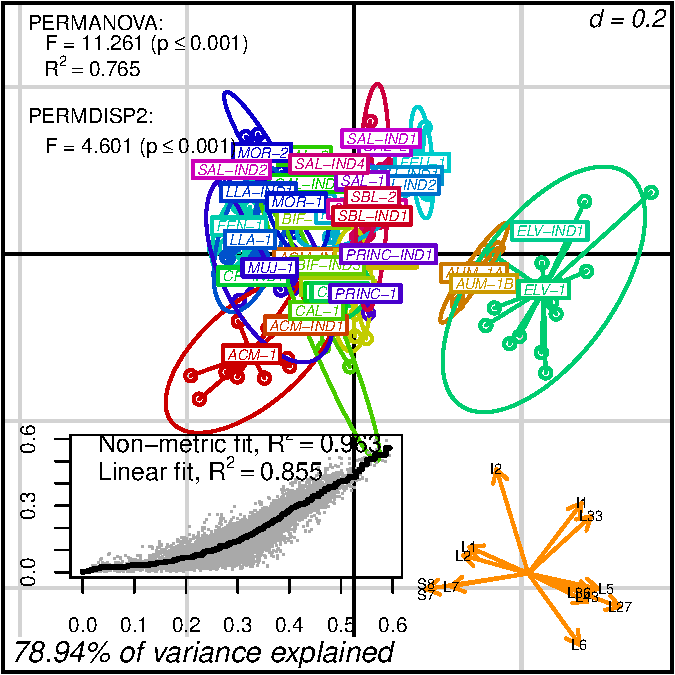
\includegraphics{_main_files/figure-latex/unnamed-chunk-67-1.pdf}
\caption{\label{fig:unnamed-chunk-67}protocol 2b}
\end{figure}

\pagebreak

\hypertarget{biplot-3d-1}{%
\subsection{Biplot 3D}\label{biplot-3d-1}}

\begin{Shaded}
\begin{Highlighting}[]
\NormalTok{biplot2d3d}\OperatorTok{::}\KeywordTok{biplot_3d}\NormalTok{(prot2a_3d,}
                      \DataTypeTok{ordination_method =} \StringTok{"PCoA"}\NormalTok{,}
                      \DataTypeTok{point_type =} \StringTok{"point"}\NormalTok{,}
                      \DataTypeTok{groups =}\NormalTok{ factor_list}\OperatorTok{$}\NormalTok{FabricGroup,}
                      \DataTypeTok{group_color =}\NormalTok{ color_list}\OperatorTok{$}\NormalTok{FabricGroup,}
                      \DataTypeTok{group_representation =} \StringTok{"stars"}\NormalTok{,}
                      \DataTypeTok{star_centroid_radius =} \DecValTok{0}\NormalTok{,}
                      \DataTypeTok{star_label_cex =} \FloatTok{.8}\NormalTok{,}
                      \DataTypeTok{arrow_min_dist =} \FloatTok{.5}\NormalTok{,}
                      \DataTypeTok{arrow_body_length =} \FloatTok{.025}\NormalTok{,}
                      \DataTypeTok{subtitle =}\NormalTok{ prot2a_3d}\OperatorTok{$}\NormalTok{sub3D,}
                      \DataTypeTok{test_text =}\NormalTok{ prot2a_tests}\OperatorTok{$}\KeywordTok{text}\NormalTok{(prot2a_tests),}
                      \DataTypeTok{test_cex =} \FloatTok{1.25}\NormalTok{,}
                      \DataTypeTok{test_fig =} \KeywordTok{c}\NormalTok{(}\DecValTok{0}\NormalTok{, }\FloatTok{0.5}\NormalTok{, }\FloatTok{0.65}\NormalTok{, }\FloatTok{.99}\NormalTok{),}
                      \DataTypeTok{view_zoom =} \FloatTok{0.9}\NormalTok{)}

\NormalTok{biplot2d3d}\OperatorTok{::}\KeywordTok{animation}\NormalTok{(}\DataTypeTok{directory =}\NormalTok{ directories}\OperatorTok{$}\NormalTok{prot2,}
                      \DataTypeTok{file_name =} \StringTok{"Prot2a_Biplot3D"}\NormalTok{)}
\end{Highlighting}
\end{Shaded}

NOTE: Animated GIF will not be displayed in the pdf version of this document.

\pagebreak

\begin{Shaded}
\begin{Highlighting}[]
\NormalTok{biplot2d3d}\OperatorTok{::}\KeywordTok{biplot_3d}\NormalTok{(prot2b_3d,}
                      \DataTypeTok{ordination_method =} \StringTok{"NMDS"}\NormalTok{,}
                      \DataTypeTok{point_type =} \StringTok{"point"}\NormalTok{,}
                      \DataTypeTok{groups =}\NormalTok{ factor_list}\OperatorTok{$}\NormalTok{FabricGroup,}
                      \DataTypeTok{group_color =}\NormalTok{ color_list}\OperatorTok{$}\NormalTok{FabricGroup,}
                      \DataTypeTok{group_representation =} \StringTok{"stars"}\NormalTok{,}
                      \DataTypeTok{star_centroid_radius =} \DecValTok{0}\NormalTok{,}
                      \DataTypeTok{star_label_cex =} \FloatTok{.8}\NormalTok{,}
                      \DataTypeTok{arrow_min_dist =} \FloatTok{.5}\NormalTok{,}
                      \DataTypeTok{arrow_body_length =} \FloatTok{.025}\NormalTok{,}
                      \DataTypeTok{subtitle =}\NormalTok{ prot2b_3d}\OperatorTok{$}\NormalTok{sub3D,}
                      \DataTypeTok{test_text =}\NormalTok{ prot2b_tests}\OperatorTok{$}\KeywordTok{text}\NormalTok{(prot2b_tests),}
                      \DataTypeTok{test_cex =} \FloatTok{1.25}\NormalTok{,}
                      \DataTypeTok{test_fig =} \KeywordTok{c}\NormalTok{(}\DecValTok{0}\NormalTok{, }\FloatTok{0.5}\NormalTok{, }\FloatTok{0.65}\NormalTok{, }\FloatTok{.99}\NormalTok{),}
                      \DataTypeTok{view_zoom =} \FloatTok{0.9}\NormalTok{)}

\NormalTok{biplot2d3d}\OperatorTok{::}\KeywordTok{animation}\NormalTok{(}\DataTypeTok{directory =}\NormalTok{ directories}\OperatorTok{$}\NormalTok{prot2,}
                      \DataTypeTok{file_name =} \StringTok{"Prot2b_Biplot3D"}\NormalTok{)}
\end{Highlighting}
\end{Shaded}

NOTE: Animated GIF will not be displayed in the pdf version of this document.

\hypertarget{prot3}{%
\chapter{Protocol 3 - Geochemical and petrographic data}\label{prot3}}

The following example applies protocol 3 to confirm workshops' provenance groups.

Protocol 3 consist in:

\begin{enumerate}
\def\labelenumi{\arabic{enumi}.}
\tightlist
\item
  Select \textbf{\emph{geochemical}} compositional data (CoDa) and ordinal \textbf{\emph{petrographic}} data;
\item
  \textbf{\emph{Centred log-ratio transformation}} (clr) and transform to \textbf{\emph{ranks}};
\item
  \textbf{\emph{Extended Gower distance}}, using \textbf{Relative ranking difference} (RRD);
\item
  Apply \textbf{\emph{Principal Coordinates Analysis}} (PCoA);
\item
  Perform \textbf{\emph{PERMANOVA \& PERMDISP}} tests;
\end{enumerate}

Last, search for outliers and re-do protocol excluding outliers.

NOTE: The \protect\hyperlink{init}{initial procedures} must be ran at least once before any protocol can be applied.

See \protect\hyperlink{prot2}{protocol 2}, for consulting references on the extended Gower distance.

\hypertarget{ordination-procedure-2}{%
\section{Ordination procedure}\label{ordination-procedure-2}}

Protocol 3 performs PCoA on a distance matrix calculated with Extended Gower coefficient of dissimilarity, combining Euclidean distances on transformed compositional data (50\%) and RRD on ranked petrographic data (50\%). As in protocol 2, PCoA requires specifying the number of dimensions and so you must 2D and 3D ordination objects separately:

\begin{Shaded}
\begin{Highlighting}[]
\NormalTok{prot3_2d <-}\StringTok{ }\KeywordTok{apply_ordination}\NormalTok{(cleanAmphorae[}\OperatorTok{!}\NormalTok{isShipwreck,], }\CommentTok{# no shipwrecks}
                             \StringTok{"3"}\NormalTok{, }\CommentTok{# select protocol 3}
                             \DataTypeTok{exception_columns =}\NormalTok{ excep_cols,}
                             \DataTypeTok{variable_tags =}\NormalTok{ varCode,}
                             \DataTypeTok{coda_override =}\NormalTok{ chemVars16,}
                             \DataTypeTok{coda_transformation_method =} \StringTok{"CLR"}\NormalTok{)}

\NormalTok{prot3_3d <-}\StringTok{ }\KeywordTok{apply_ordination}\NormalTok{(cleanAmphorae[}\OperatorTok{!}\NormalTok{isShipwreck,], }\CommentTok{# no shipwrecks}
                             \StringTok{"3"}\NormalTok{, }\CommentTok{# select protocol 3}
                             \DataTypeTok{exception_columns =}\NormalTok{ excep_cols,}
                             \DataTypeTok{variable_tags =}\NormalTok{ varCode,}
                             \DataTypeTok{coda_override =}\NormalTok{ chemVars16,}
                             \DataTypeTok{coda_transformation =} \StringTok{"CLR"}\NormalTok{,}
                             \DataTypeTok{dimensions =} \DecValTok{3}\NormalTok{)}
\end{Highlighting}
\end{Shaded}

\hypertarget{simplify-coda-names-1}{%
\section{Simplify CoDa names}\label{simplify-coda-names-1}}

We may want to simplify the names of the transformed variables before plotting them in a biplot.

\begin{Shaded}
\begin{Highlighting}[]
\NormalTok{prot3_2d <-}\StringTok{ }\KeywordTok{simplify_coda_names}\NormalTok{(prot3_2d)}
\NormalTok{prot3_3d <-}\StringTok{ }\KeywordTok{simplify_coda_names}\NormalTok{(prot3_3d)}
\end{Highlighting}
\end{Shaded}

\hypertarget{test-the-given-provenance-groups}{%
\section{Test the given provenance groups}\label{test-the-given-provenance-groups}}

Because protocol 3 uses both geochemical and petrographic information, we can test the provenance assigned to the amphorae samples.

\begin{Shaded}
\begin{Highlighting}[]
\NormalTok{prot3_tests <-}\StringTok{ }\KeywordTok{test_groups}\NormalTok{(prot3_2d}\OperatorTok{$}\NormalTok{dist_matrix, }
\NormalTok{                           factor_list}\OperatorTok{$}\NormalTok{ProvGroup)}
\CommentTok{#> [1] "initiating test batch..."}
\CommentTok{#> [1] "vegan::anosim done."}
\CommentTok{#> [1] "vegan::betadisper done."}
\CommentTok{#> [1] "vegan::permutest done."}
\CommentTok{#> [1] "vegan::adonis done."}
\CommentTok{#> [1] "Test batch completed."}
\end{Highlighting}
\end{Shaded}

These tests were explained in \protect\hyperlink{tests}{protocol 1}.

\pagebreak

\hypertarget{biplots-1}{%
\section{Biplots}\label{biplots-1}}

The details on how to create biplots is already explained in \protect\hyperlink{biplot}{protocol 1}. Unlike protocol 2, protocol 3 only generates one kind of projection (RRD, PCoA).

\hypertarget{biplot-2d-2}{%
\subsection{Biplot 2D}\label{biplot-2d-2}}

\begin{Shaded}
\begin{Highlighting}[]
\NormalTok{arrows_label_adj <-}\StringTok{ }\KeywordTok{rbind}\NormalTok{(}\KeywordTok{c}\NormalTok{(.}\DecValTok{5}\NormalTok{,.}\DecValTok{8}\NormalTok{),}\KeywordTok{c}\NormalTok{(.}\DecValTok{5}\NormalTok{,}\DecValTok{1}\NormalTok{),}\KeywordTok{c}\NormalTok{(.}\DecValTok{5}\NormalTok{,}\DecValTok{1}\NormalTok{),}\KeywordTok{c}\NormalTok{(.}\DecValTok{5}\NormalTok{,}\DecValTok{0}\NormalTok{),}\KeywordTok{c}\NormalTok{(.}\DecValTok{5}\NormalTok{,}\DecValTok{1}\NormalTok{),}
                          \KeywordTok{c}\NormalTok{(.}\DecValTok{5}\NormalTok{,}\DecValTok{0}\NormalTok{),}\KeywordTok{c}\NormalTok{(}\DecValTok{0}\NormalTok{,.}\DecValTok{5}\NormalTok{))}
\KeywordTok{row.names}\NormalTok{(arrows_label_adj) <-}\StringTok{ }\KeywordTok{c}\NormalTok{(}\StringTok{"L48"}\NormalTok{,}\StringTok{"L24"}\NormalTok{,}\StringTok{"L5"}\NormalTok{,}\StringTok{"L36"}\NormalTok{,}\StringTok{"S7"}\NormalTok{,}
                                 \StringTok{"S8"}\NormalTok{,}\StringTok{"S11"}\NormalTok{)}

\NormalTok{biplot2d3d}\OperatorTok{::}\KeywordTok{biplot_2d}\NormalTok{(prot3_2d,}
                      \DataTypeTok{ordination_method =} \StringTok{"PCoA"}\NormalTok{,}
                      \DataTypeTok{invert_coordinates =} \KeywordTok{c}\NormalTok{ (}\OtherTok{TRUE}\NormalTok{,}\OtherTok{TRUE}\NormalTok{),}
                      \DataTypeTok{ylim =} \KeywordTok{c}\NormalTok{(}\OperatorTok{-}\NormalTok{.}\DecValTok{3}\NormalTok{,.}\DecValTok{29}\NormalTok{),}
                      \DataTypeTok{point_type =} \StringTok{"point"}\NormalTok{,}
                      \DataTypeTok{groups =}\NormalTok{ factor_list}\OperatorTok{$}\NormalTok{FabricGroup,}
                      \DataTypeTok{group_color =}\NormalTok{ color_list}\OperatorTok{$}\NormalTok{FabricGroup,}
                      \DataTypeTok{group_label_cex =} \FloatTok{0.6}\NormalTok{,}
                      \DataTypeTok{arrow_mim_dist =} \FloatTok{0.5}\NormalTok{,}
                      \DataTypeTok{arrow_label_cex =} \FloatTok{0.6}\NormalTok{,}
                      \DataTypeTok{arrow_fig =} \KeywordTok{c}\NormalTok{(.}\DecValTok{6}\NormalTok{,.}\DecValTok{95}\NormalTok{,}\DecValTok{0}\NormalTok{,.}\DecValTok{35}\NormalTok{),}
                      \DataTypeTok{arrow_label_adj_override =}\NormalTok{ arrows_label_adj,}
                      \DataTypeTok{subtitle =}\NormalTok{ prot3_2d}\OperatorTok{$}\NormalTok{sub2D,}
                      \DataTypeTok{test_text =}\NormalTok{ prot3_tests}\OperatorTok{$}\KeywordTok{text}\NormalTok{(prot3_tests),}
                      \DataTypeTok{test_cex =} \FloatTok{0.8}\NormalTok{,}
                      \DataTypeTok{test_fig =} \KeywordTok{c}\NormalTok{(}\DecValTok{0}\NormalTok{, }\FloatTok{0.5}\NormalTok{, }\FloatTok{0.65}\NormalTok{, }\FloatTok{.99}\NormalTok{),}
                      \DataTypeTok{fitAnalysis_fig =} \KeywordTok{c}\NormalTok{(}\DecValTok{0}\NormalTok{,.}\DecValTok{7}\NormalTok{,.}\DecValTok{05}\NormalTok{,.}\DecValTok{5}\NormalTok{),}
                      \DataTypeTok{output_type =} \StringTok{"preview"}\NormalTok{)}
\end{Highlighting}
\end{Shaded}

\begin{figure}
\centering
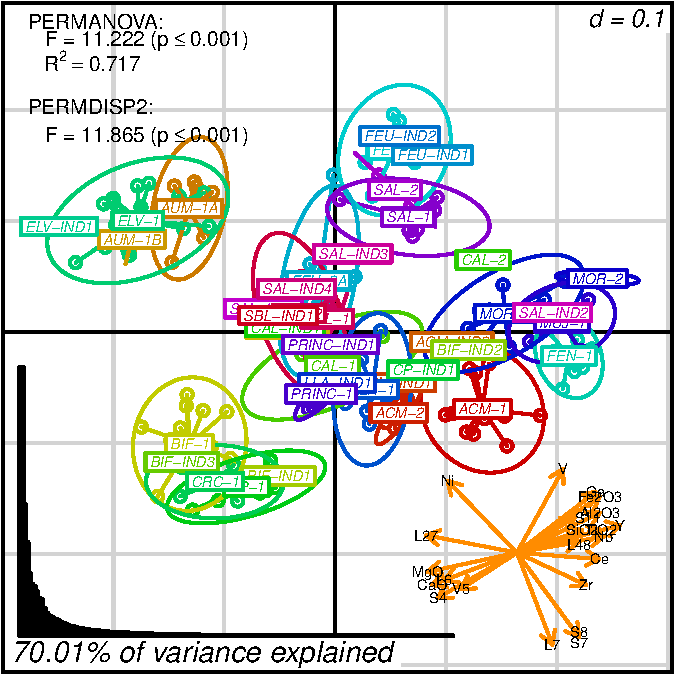
\includegraphics{_main_files/figure-latex/unnamed-chunk-75-1.pdf}
\caption{\label{fig:unnamed-chunk-75}protocol 3}
\end{figure}

\pagebreak

\hypertarget{biplot-3d-2}{%
\subsection{Biplot 3D}\label{biplot-3d-2}}

\begin{Shaded}
\begin{Highlighting}[]
\NormalTok{biplot2d3d}\OperatorTok{::}\KeywordTok{biplot_3d}\NormalTok{(prot3_3d,}
                      \DataTypeTok{ordination_method =} \StringTok{"PCoA"}\NormalTok{,}
                      \DataTypeTok{point_type =} \StringTok{"point"}\NormalTok{,}
                      \DataTypeTok{groups =}\NormalTok{ factor_list}\OperatorTok{$}\NormalTok{FabricGroup,}
                      \DataTypeTok{group_color =}\NormalTok{ color_list}\OperatorTok{$}\NormalTok{FabricGroup,}
                      \DataTypeTok{group_representation =} \StringTok{"stars"}\NormalTok{,}
                      \DataTypeTok{star_centroid_radius =} \DecValTok{0}\NormalTok{,}
                      \DataTypeTok{star_label_cex =} \FloatTok{.8}\NormalTok{,}
                      \DataTypeTok{arrow_min_dist =} \FloatTok{.5}\NormalTok{,}
                      \DataTypeTok{arrow_body_length =} \FloatTok{.025}\NormalTok{,}
                      \DataTypeTok{subtitle =}\NormalTok{ prot3_3d}\OperatorTok{$}\NormalTok{sub3D,}
                      \DataTypeTok{test_text =}\NormalTok{ prot3_tests}\OperatorTok{$}\KeywordTok{text}\NormalTok{(prot3_tests),}
                      \DataTypeTok{test_cex =} \FloatTok{1.25}\NormalTok{,}
                      \DataTypeTok{test_fig =} \KeywordTok{c}\NormalTok{(}\DecValTok{0}\NormalTok{, }\FloatTok{0.5}\NormalTok{, }\FloatTok{0.65}\NormalTok{, }\FloatTok{.99}\NormalTok{),}
                      \DataTypeTok{view_zoom =} \FloatTok{0.9}\NormalTok{)}

\NormalTok{biplot2d3d}\OperatorTok{::}\KeywordTok{animation}\NormalTok{(}\DataTypeTok{directory =}\NormalTok{ directories}\OperatorTok{$}\NormalTok{prot3,}
                      \DataTypeTok{file_name =} \StringTok{"Prot3_Biplot3D"}\NormalTok{)}
\end{Highlighting}
\end{Shaded}

NOTE: Animated GIF will not be displayed in the pdf version of this document.

\hypertarget{prot4}{%
\chapter{Protocol 4 - Provenance data}\label{prot4}}

The following example applies protocol 4 to confirm workshops' provenance groups.

Protocol 4 consist in:

\begin{enumerate}
\def\labelenumi{\arabic{enumi}.}
\tightlist
\item
  Select provenance-specific variables in \textbf{\emph{geochemical}} compositional data (CoDa) and ordinal \textbf{\emph{petrographic}} data;
\item
  \textbf{\emph{Centred log-ratio transformation}} (clr) and transform to \textbf{\emph{ranks}};
\item
  \textbf{\emph{Extended Gower coefficient of dissimilarity}}, using \textbf{Relative ranking difference} (RRD);
\item
  Apply \textbf{\emph{Principal Coordinates Analysis}} (PCoA);
\item
  Perform \textbf{\emph{PERMANOVA \& PERMDISP}} tests;
\end{enumerate}

Last, search for outliers and re-do protocol excluding outliers.

NOTE: The \protect\hyperlink{init}{initial procedures} must be ran at least once before any protocol can be applied.

\hypertarget{ordination-procedure-3}{%
\section{Ordination procedure}\label{ordination-procedure-3}}

As protocol 3, protocol 4 performs PCoA on a distance matrix calculated with Extended Gower coefficient of dissimilarity, combining Euclidean distances on transformed compositional data (50\%) and RRD on ranked petrographic data (50\%).

\begin{Shaded}
\begin{Highlighting}[]
\NormalTok{prot4_2d <-}\StringTok{ }\KeywordTok{apply_ordination}\NormalTok{(cleanAmphorae[}\OperatorTok{!}\NormalTok{isShipwreck,],}
                             \StringTok{"4"}\NormalTok{, }\CommentTok{# select protocol 4}
                             \DataTypeTok{exception_columns =}\NormalTok{ excep_cols,}
                             \DataTypeTok{variable_tags =}\NormalTok{ varCode,}
                             \DataTypeTok{coda_override =}\NormalTok{ chemVars16,}
                             \DataTypeTok{coda_transformation_method =} \StringTok{"CLR"}\NormalTok{)}

\NormalTok{prot4_3d <-}\StringTok{ }\KeywordTok{apply_ordination}\NormalTok{(cleanAmphorae[}\OperatorTok{!}\NormalTok{isShipwreck,],}
                             \StringTok{"4"}\NormalTok{, }\CommentTok{# select protocol 4}
                             \DataTypeTok{exception_columns =}\NormalTok{ excep_cols,}
                             \DataTypeTok{variable_tags =}\NormalTok{ varCode,}
                             \DataTypeTok{coda_override =}\NormalTok{ chemVars16,}
                             \DataTypeTok{coda_transformation_method =} \StringTok{"CLR"}\NormalTok{,}
                             \DataTypeTok{dimensions =} \DecValTok{3}\NormalTok{)}
\end{Highlighting}
\end{Shaded}

However, protocol 4 uses a finer selection of petrographic variables, which are considered indicative of provenance (raw materials) rather than technology. Compare the number of variables in protocol 3 and 4:

\begin{tabular}{r|r}
\hline
Protocol 3 & Protocol 4\\
\hline
78 & 59\\
\hline
\end{tabular}

\hypertarget{simplify-coda-names-2}{%
\section{Simplify CoDa names}\label{simplify-coda-names-2}}

We may want to simplify the names of the transformed variables before plotting them in a biplot.

\begin{Shaded}
\begin{Highlighting}[]
\NormalTok{prot4_2d <-}\StringTok{ }\KeywordTok{simplify_coda_names}\NormalTok{(prot4_2d)}
\NormalTok{prot4_3d <-}\StringTok{ }\KeywordTok{simplify_coda_names}\NormalTok{(prot4_3d)}
\end{Highlighting}
\end{Shaded}

\hypertarget{test-the-given-provenance-groups-1}{%
\section{Test the given provenance groups}\label{test-the-given-provenance-groups-1}}

With protocol 4, we can test the provenance assigned to the amphorae samples based only on provenance-specific variables.

\begin{Shaded}
\begin{Highlighting}[]
\NormalTok{prot4_tests <-}\StringTok{ }\KeywordTok{test_groups}\NormalTok{(prot4_2d}\OperatorTok{$}\NormalTok{dist_matrix,}
\NormalTok{                           factor_list}\OperatorTok{$}\NormalTok{ProvGroup)}
\CommentTok{#> [1] "initiating test batch..."}
\CommentTok{#> [1] "vegan::anosim done."}
\CommentTok{#> [1] "vegan::betadisper done."}
\CommentTok{#> [1] "vegan::permutest done."}
\CommentTok{#> [1] "vegan::adonis done."}
\CommentTok{#> [1] "Test batch completed."}
\end{Highlighting}
\end{Shaded}

These tests were explained in \protect\hyperlink{tests}{protocol 1}.

\pagebreak

\hypertarget{biplots-2}{%
\section{Biplots}\label{biplots-2}}

The details on how to create biplots is already explained in \protect\hyperlink{biplot}{protocol 1}. As protocol 3, protocol 4 only generates one kind of projection (RRD, PCoA).

\hypertarget{biplot-2d-3}{%
\subsection{Biplot 2D}\label{biplot-2d-3}}

\begin{Shaded}
\begin{Highlighting}[]
\NormalTok{arrows_label_adj <-}\StringTok{ }\KeywordTok{rbind}\NormalTok{(}\KeywordTok{c}\NormalTok{(.}\DecValTok{5}\NormalTok{,}\DecValTok{1}\NormalTok{),}\KeywordTok{c}\NormalTok{(}\DecValTok{0}\NormalTok{,}\DecValTok{0}\NormalTok{),}\KeywordTok{c}\NormalTok{(}\DecValTok{1}\NormalTok{,.}\DecValTok{5}\NormalTok{),}\KeywordTok{c}\NormalTok{(}\DecValTok{0}\NormalTok{,}\DecValTok{1}\NormalTok{),}\KeywordTok{c}\NormalTok{(}\DecValTok{1}\NormalTok{,}\DecValTok{0}\NormalTok{),}
                          \KeywordTok{c}\NormalTok{(}\DecValTok{0}\NormalTok{,.}\DecValTok{5}\NormalTok{),}\KeywordTok{c}\NormalTok{(.}\DecValTok{5}\NormalTok{,}\DecValTok{1}\NormalTok{),}\KeywordTok{c}\NormalTok{(}\DecValTok{1}\NormalTok{,.}\DecValTok{5}\NormalTok{),}\KeywordTok{c}\NormalTok{(.}\DecValTok{5}\NormalTok{,}\DecValTok{1}\NormalTok{))}
\KeywordTok{row.names}\NormalTok{(arrows_label_adj) <-}\StringTok{ }\KeywordTok{c}\NormalTok{(}\StringTok{"CaO"}\NormalTok{,}\StringTok{"S4"}\NormalTok{,}\StringTok{"S7"}\NormalTok{,}\StringTok{"S8"}\NormalTok{,}\StringTok{"Ce"}\NormalTok{,}
                                 \StringTok{"Nb"}\NormalTok{,}\StringTok{"Al2O3"}\NormalTok{,}\StringTok{"S11"}\NormalTok{,}\StringTok{"Fe2O3"}\NormalTok{)}

\NormalTok{biplot2d3d}\OperatorTok{::}\KeywordTok{biplot_2d}\NormalTok{(prot4_2d,}
                      \DataTypeTok{ordination_method =} \StringTok{"PCoA"}\NormalTok{,}
                      \DataTypeTok{invert_coordinates =} \KeywordTok{c}\NormalTok{ (}\OtherTok{TRUE}\NormalTok{,}\OtherTok{FALSE}\NormalTok{),}
                      \DataTypeTok{ylim =} \KeywordTok{c}\NormalTok{(}\OperatorTok{-}\NormalTok{.}\DecValTok{35}\NormalTok{,.}\DecValTok{32}\NormalTok{),}
                      \DataTypeTok{point_type =} \StringTok{"point"}\NormalTok{,}
                      \DataTypeTok{groups =}\NormalTok{ factor_list}\OperatorTok{$}\NormalTok{ProvGroup,}
                      \DataTypeTok{group_color =}\NormalTok{ color_list}\OperatorTok{$}\NormalTok{ProvGroup,}
                      \DataTypeTok{group_label_cex =} \FloatTok{0.6}\NormalTok{,}
                      \DataTypeTok{arrow_mim_dist =} \FloatTok{.5}\NormalTok{,}
                      \DataTypeTok{arrow_label_cex =} \FloatTok{0.6}\NormalTok{,}
                      \DataTypeTok{arrow_fig =} \KeywordTok{c}\NormalTok{(.}\DecValTok{6}\NormalTok{,.}\DecValTok{95}\NormalTok{,}\DecValTok{0}\NormalTok{,.}\DecValTok{35}\NormalTok{),}
                      \DataTypeTok{arrow_label_adj_override =}\NormalTok{ arrows_label_adj,}
                      \DataTypeTok{subtitle =}\NormalTok{ prot4_2d}\OperatorTok{$}\NormalTok{sub2D,}
                      \DataTypeTok{test_text =}\NormalTok{ prot4_tests}\OperatorTok{$}\KeywordTok{text}\NormalTok{(prot4_tests),}
                      \DataTypeTok{test_cex =} \FloatTok{0.8}\NormalTok{,}
                      \DataTypeTok{test_fig =} \KeywordTok{c}\NormalTok{(}\DecValTok{0}\NormalTok{, }\FloatTok{0.5}\NormalTok{, }\FloatTok{0.62}\NormalTok{, }\FloatTok{.99}\NormalTok{),}
                      \DataTypeTok{fitAnalysis_fig =} \KeywordTok{c}\NormalTok{(}\DecValTok{0}\NormalTok{,.}\DecValTok{7}\NormalTok{,.}\DecValTok{05}\NormalTok{,.}\DecValTok{5}\NormalTok{),}
                      \DataTypeTok{output_type =} \StringTok{"preview"}\NormalTok{)}
\end{Highlighting}
\end{Shaded}

\begin{figure}
\centering
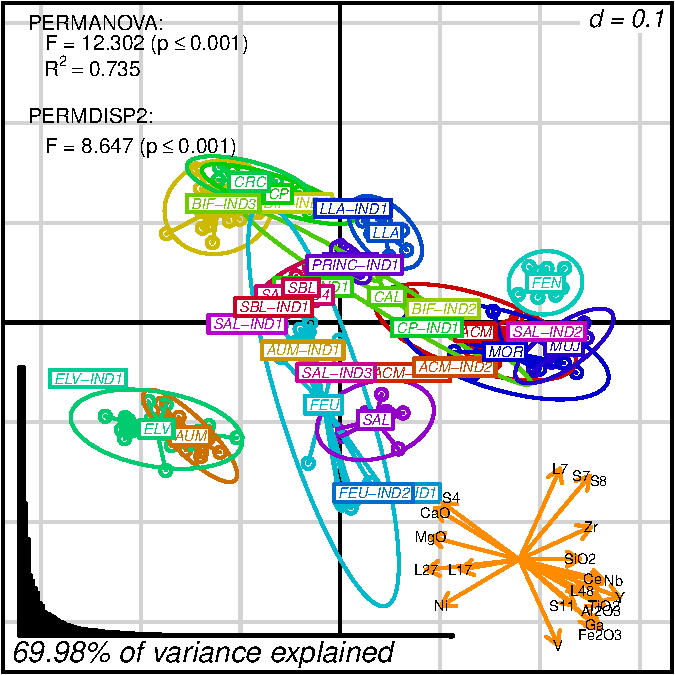
\includegraphics{_main_files/figure-latex/unnamed-chunk-84-1.pdf}
\caption{\label{fig:unnamed-chunk-84}protocol 4}
\end{figure}

\pagebreak

\hypertarget{biplot-3d-3}{%
\subsection{Biplot 3D}\label{biplot-3d-3}}

\begin{Shaded}
\begin{Highlighting}[]
\NormalTok{biplot2d3d}\OperatorTok{::}\KeywordTok{biplot_3d}\NormalTok{(prot4_3d,}
                      \DataTypeTok{ordination_method =} \StringTok{"PCoA"}\NormalTok{,}
                      \DataTypeTok{point_type =} \StringTok{"point"}\NormalTok{,}
                      \DataTypeTok{groups =}\NormalTok{ factor_list}\OperatorTok{$}\NormalTok{FabricGroup,}
                      \DataTypeTok{group_color =}\NormalTok{ color_list}\OperatorTok{$}\NormalTok{FabricGroup,}
                      \DataTypeTok{group_representation =} \StringTok{"stars"}\NormalTok{,}
                      \DataTypeTok{star_centroid_radius =} \DecValTok{0}\NormalTok{,}
                      \DataTypeTok{star_label_cex =} \FloatTok{.8}\NormalTok{,}
                      \DataTypeTok{arrow_min_dist =} \FloatTok{.5}\NormalTok{,}
                      \DataTypeTok{arrow_body_length =} \FloatTok{.025}\NormalTok{,}
                      \DataTypeTok{subtitle =}\NormalTok{ prot4_3d}\OperatorTok{$}\NormalTok{sub3D,}
                      \DataTypeTok{test_text =}\NormalTok{ prot4_tests}\OperatorTok{$}\KeywordTok{text}\NormalTok{(prot4_tests),}
                      \DataTypeTok{test_cex =} \FloatTok{1.25}\NormalTok{,}
                      \DataTypeTok{test_fig =} \KeywordTok{c}\NormalTok{(}\DecValTok{0}\NormalTok{, }\FloatTok{0.5}\NormalTok{, }\FloatTok{0.65}\NormalTok{, }\FloatTok{.99}\NormalTok{),}
                      \DataTypeTok{view_zoom =} \FloatTok{0.9}\NormalTok{)}

\NormalTok{biplot2d3d}\OperatorTok{::}\KeywordTok{animation}\NormalTok{(}\DataTypeTok{directory =}\NormalTok{ directories}\OperatorTok{$}\NormalTok{prot4,}
                       \DataTypeTok{file_name =} \StringTok{"Prot4_Biplot3D"}\NormalTok{)}
\end{Highlighting}
\end{Shaded}

NOTE: Animated GIF will not be displayed in the pdf version of this document.

\hypertarget{prot4_ship}{%
\chapter{Protocol 4 - Provenance data with shipwrecks}\label{prot4_ship}}

The following example applies protocol 4 to confirm shipwrecks samples attribution to workshops' provenance groups.

Protocol 4 consist in:

\begin{enumerate}
\def\labelenumi{\arabic{enumi}.}
\tightlist
\item
  Select provenance-specific variables in \textbf{\emph{geochemical}} compositional data (CoDa) and ordinal \textbf{\emph{petrographic}} data;
\item
  \textbf{\emph{Centred log-ratio transformation}} (clr) and transform to \textbf{\emph{ranks}};
\item
  \textbf{\emph{Extended Gower coefficient of dissimilarity}}, using \textbf{Relative ranking difference} (RRD);
\item
  Apply \textbf{\emph{Principal Coordinates Analysis}} (PCoA);
\item
  Perform \textbf{\emph{PERMANOVA \& PERMDISP}} tests;
\end{enumerate}

Last, search for outliers and re-do protocol excluding outliers.

NOTE: The \protect\hyperlink{init}{initial procedures} must be ran at least once before any protocol can be applied.

\hypertarget{ordination-procedure-4}{%
\section{Ordination procedure}\label{ordination-procedure-4}}

As protocol 3, protocol 4 performs PCoA on a distance matrix calculated with Extended Gower coefficient of dissimilarity, combining Euclidean distances on transformed compositional data (50\%) and RRD on ranked petrographic data (50\%). In this case, we are not filtering out the shipwreck samples, but we do exclude the true outliers (IND, observations with no group assigned) so they don't pollute visualization.

\begin{Shaded}
\begin{Highlighting}[]
\NormalTok{prot4_Shipwreck_2d <-}\StringTok{ }\KeywordTok{apply_ordination}\NormalTok{(}\CommentTok{# no true outliers}
\NormalTok{                                       cleanAmphorae[}\OperatorTok{!}\NormalTok{isTrueIND,],}
                                       \StringTok{"4"}\NormalTok{, }\CommentTok{# select protocol 4}
                                       \DataTypeTok{exception_columns =}\NormalTok{ excep_cols,}
                                       \DataTypeTok{variable_tags =}\NormalTok{ varCode,}
                                       \DataTypeTok{coda_override =}\NormalTok{ chemVars16,}
                                       \DataTypeTok{coda_transformation_method =} \StringTok{"CLR"}\NormalTok{)}

\NormalTok{prot4_Shipwreck_3d <-}\StringTok{ }\KeywordTok{apply_ordination}\NormalTok{(}\CommentTok{# no true outliers}
\NormalTok{                                       cleanAmphorae[}\OperatorTok{!}\NormalTok{isTrueIND,],}
                                       \StringTok{"4"}\NormalTok{, }\CommentTok{# select protocol 4}
                                       \DataTypeTok{exception_columns =}\NormalTok{ excep_cols,}
                                       \DataTypeTok{variable_tags =}\NormalTok{ varCode,}
                                       \DataTypeTok{coda_override =}\NormalTok{ chemVars16,}
                                       \DataTypeTok{coda_transformation_method =} \StringTok{"CLR"}\NormalTok{,}
                                       \DataTypeTok{dimensions =} \DecValTok{3}\NormalTok{)}
\end{Highlighting}
\end{Shaded}

\hypertarget{simplify-coda-names-3}{%
\section{Simplify CoDa names}\label{simplify-coda-names-3}}

We may want to simplify the names of the transformed variables before plotting them in a biplot.

\begin{Shaded}
\begin{Highlighting}[]
\NormalTok{prot4_Shipwreck_2d <-}\StringTok{ }\KeywordTok{simplify_coda_names}\NormalTok{(prot4_Shipwreck_2d)}
\NormalTok{prot4_Shipwreck_3d <-}\StringTok{ }\KeywordTok{simplify_coda_names}\NormalTok{(prot4_Shipwreck_3d)}
\end{Highlighting}
\end{Shaded}

\hypertarget{test-the-given-provenance-groups-2}{%
\section{Test the given provenance groups}\label{test-the-given-provenance-groups-2}}

We can test the provenance assigned to shipwrecks' amphorae samples together with those found and assigned to the workshops.

\begin{Shaded}
\begin{Highlighting}[]
\NormalTok{prot4_Shipwreck_tests <-}\StringTok{ }\KeywordTok{test_groups}\NormalTok{(prot4_Shipwreck_2d}\OperatorTok{$}\NormalTok{dist_matrix,}
\NormalTok{                                     factor_list_Shipwreck}\OperatorTok{$}\NormalTok{ProvGroup)}
\CommentTok{#> [1] "initiating test batch..."}
\CommentTok{#> [1] "vegan::anosim done."}
\CommentTok{#> [1] "vegan::betadisper done."}
\CommentTok{#> [1] "vegan::permutest done."}
\CommentTok{#> [1] "vegan::adonis done."}
\CommentTok{#> [1] "Test batch completed."}
\end{Highlighting}
\end{Shaded}

These tests were explained in \href{3_prot1.html}{protocol 1}.

\pagebreak

\hypertarget{biplots-3}{%
\section{Biplots}\label{biplots-3}}

The details on how to create biplots is already explained in \protect\hyperlink{biplot}{protocol 1}. Protocol 4 generates PCoA projections.

\hypertarget{biplot-2d-4}{%
\subsection{Biplot 2D}\label{biplot-2d-4}}

\begin{Shaded}
\begin{Highlighting}[]
\NormalTok{arrows_label_adj <-}\StringTok{ }\KeywordTok{rbind}\NormalTok{(}\KeywordTok{c}\NormalTok{(.}\DecValTok{5}\NormalTok{,}\DecValTok{0}\NormalTok{),}\KeywordTok{c}\NormalTok{(.}\DecValTok{5}\NormalTok{,}\DecValTok{1}\NormalTok{),}\KeywordTok{c}\NormalTok{(.}\DecValTok{5}\NormalTok{,}\DecValTok{0}\NormalTok{),}\KeywordTok{c}\NormalTok{(.}\DecValTok{5}\NormalTok{,}\DecValTok{1}\NormalTok{),}\KeywordTok{c}\NormalTok{(.}\DecValTok{5}\NormalTok{,}\DecValTok{0}\NormalTok{),}
                          \KeywordTok{c}\NormalTok{(.}\DecValTok{5}\NormalTok{,}\DecValTok{1}\NormalTok{),}\KeywordTok{c}\NormalTok{(.}\DecValTok{8}\NormalTok{,}\DecValTok{0}\NormalTok{),}\KeywordTok{c}\NormalTok{(}\DecValTok{1}\NormalTok{,.}\DecValTok{5}\NormalTok{),}\KeywordTok{c}\NormalTok{(.}\DecValTok{5}\NormalTok{,}\DecValTok{0}\NormalTok{),}\KeywordTok{c}\NormalTok{(}\DecValTok{1}\NormalTok{,.}\DecValTok{2}\NormalTok{),}
                          \KeywordTok{c}\NormalTok{(.}\DecValTok{5}\NormalTok{,}\DecValTok{1}\NormalTok{),}\KeywordTok{c}\NormalTok{(.}\DecValTok{2}\NormalTok{,.}\DecValTok{7}\NormalTok{))}
\KeywordTok{row.names}\NormalTok{(arrows_label_adj) <-}\StringTok{ }\KeywordTok{c}\NormalTok{(}\StringTok{"S7"}\NormalTok{,}\StringTok{"S8"}\NormalTok{,}\StringTok{"S4"}\NormalTok{,}\StringTok{"CaO"}\NormalTok{,}\StringTok{"MgO"}\NormalTok{,}
                                 \StringTok{"S11"}\NormalTok{,}\StringTok{"L48"}\NormalTok{,}\StringTok{"SiO2"}\NormalTok{,}\StringTok{"Ce"}\NormalTok{,}\StringTok{"Nb"}\NormalTok{,}
                                 \StringTok{"Th"}\NormalTok{,}\StringTok{"TiO2"}\NormalTok{)}

\NormalTok{biplot2d3d}\OperatorTok{::}\KeywordTok{biplot_2d}\NormalTok{(prot4_Shipwreck_2d,}
                      \DataTypeTok{ordination_method =} \StringTok{"PCoA"}\NormalTok{,}
                      \DataTypeTok{invert_coordinates =} \KeywordTok{c}\NormalTok{ (}\OtherTok{TRUE}\NormalTok{,}\OtherTok{TRUE}\NormalTok{),}
                      \DataTypeTok{ylim =} \KeywordTok{c}\NormalTok{(}\OperatorTok{-}\NormalTok{.}\DecValTok{3}\NormalTok{,.}\DecValTok{25}\NormalTok{),}
                      \DataTypeTok{point_type =} \StringTok{"point"}\NormalTok{,}
                      \DataTypeTok{groups =}\NormalTok{ factor_list_Shipwreck}\OperatorTok{$}\NormalTok{ProvGroup,}
                      \DataTypeTok{group_color =}\NormalTok{ color_list_Shipwreck}\OperatorTok{$}\NormalTok{ProvGroup,}
                      \DataTypeTok{group_label_cex =} \FloatTok{0.6}\NormalTok{,}
                      \DataTypeTok{arrow_mim_dist =} \FloatTok{.5}\NormalTok{,}
                      \DataTypeTok{arrow_label_cex =} \FloatTok{0.6}\NormalTok{,}
                      \DataTypeTok{arrow_fig =} \KeywordTok{c}\NormalTok{(.}\DecValTok{6}\NormalTok{,.}\DecValTok{95}\NormalTok{,}\DecValTok{0}\NormalTok{,.}\DecValTok{35}\NormalTok{),}
                      \DataTypeTok{arrow_label_adj_override =}\NormalTok{ arrows_label_adj,}
                      \DataTypeTok{subtitle =}\NormalTok{ prot4_Shipwreck_2d}\OperatorTok{$}\NormalTok{sub2D,}
                      \DataTypeTok{test_text =} 
\NormalTok{                        prot4_Shipwreck_tests}\OperatorTok{$}\KeywordTok{text}\NormalTok{(prot4_Shipwreck_tests),}
                      \DataTypeTok{test_cex =} \FloatTok{0.8}\NormalTok{,}
                      \DataTypeTok{test_fig =} \KeywordTok{c}\NormalTok{(}\DecValTok{0}\NormalTok{, }\FloatTok{0.5}\NormalTok{, }\FloatTok{0.62}\NormalTok{, }\FloatTok{.99}\NormalTok{),}
                      \DataTypeTok{fitAnalysis_fig =} \KeywordTok{c}\NormalTok{(}\DecValTok{0}\NormalTok{,.}\DecValTok{7}\NormalTok{,.}\DecValTok{05}\NormalTok{,.}\DecValTok{5}\NormalTok{),}
                      \DataTypeTok{output_type =} \StringTok{"preview"}\NormalTok{)}
\end{Highlighting}
\end{Shaded}

\begin{figure}
\centering
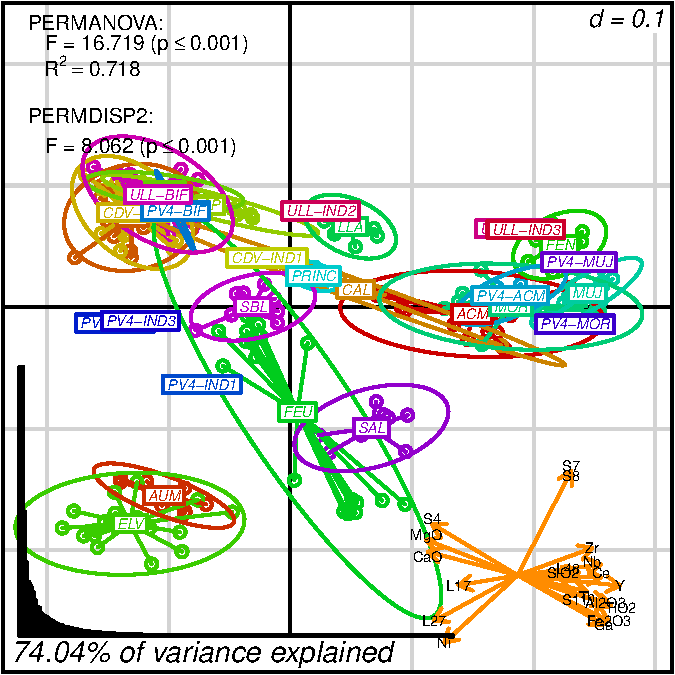
\includegraphics{_main_files/figure-latex/unnamed-chunk-91-1.pdf}
\caption{\label{fig:unnamed-chunk-91}protocol 4 with shipwrecks}
\end{figure}

\pagebreak

\hypertarget{biplot-3d-4}{%
\subsection{Biplot 3D}\label{biplot-3d-4}}

\begin{Shaded}
\begin{Highlighting}[]
\NormalTok{biplot2d3d}\OperatorTok{::}\KeywordTok{biplot_3d}\NormalTok{(prot4_Shipwreck_3d,}
                      \DataTypeTok{ordination_method =} \StringTok{"PCoA"}\NormalTok{,}
                      \DataTypeTok{point_type =} \StringTok{"point"}\NormalTok{,}
                      \DataTypeTok{groups =}\NormalTok{ factor_list_Shipwreck}\OperatorTok{$}\NormalTok{FabricGroup,}
                      \DataTypeTok{group_color =}\NormalTok{ color_list_Shipwreck}\OperatorTok{$}\NormalTok{FabricGroup,}
                      \DataTypeTok{group_representation =} \StringTok{"stars"}\NormalTok{,}
                      \DataTypeTok{star_centroid_radius =} \DecValTok{0}\NormalTok{,}
                      \DataTypeTok{star_label_cex =} \FloatTok{.8}\NormalTok{,}
                      \DataTypeTok{arrow_min_dist =} \FloatTok{.5}\NormalTok{,}
                      \DataTypeTok{arrow_body_length =} \FloatTok{.025}\NormalTok{,}
                      \DataTypeTok{subtitle =}\NormalTok{ prot4_Shipwreck_3d}\OperatorTok{$}\NormalTok{sub3D,}
                      \DataTypeTok{test_text =} 
\NormalTok{                        prot4_Shipwreck_tests}\OperatorTok{$}\KeywordTok{text}\NormalTok{(prot4_Shipwreck_tests),}
                      \DataTypeTok{test_cex =} \FloatTok{1.25}\NormalTok{,}
                      \DataTypeTok{test_fig =} \KeywordTok{c}\NormalTok{(}\DecValTok{0}\NormalTok{, }\FloatTok{0.5}\NormalTok{, }\FloatTok{0.65}\NormalTok{, }\FloatTok{.99}\NormalTok{),}
                      \DataTypeTok{view_zoom =} \FloatTok{0.9}\NormalTok{)}

\NormalTok{biplot2d3d}\OperatorTok{::}\KeywordTok{animation}\NormalTok{(}\DataTypeTok{directory =}\NormalTok{ directories}\OperatorTok{$}\NormalTok{prot4_Shipwreck,}
                       \DataTypeTok{file_name =} \StringTok{"Prot4_Shipwreck_Biplot3D"}\NormalTok{)}
\end{Highlighting}
\end{Shaded}

NOTE: Animated GIF will not be displayed in the pdf version of this document.

\hypertarget{interp_biplots}{%
\chapter{Interpreting biplots}\label{interp_biplots}}

This section is a reminder of the possible caveats of interpreting multivariate projections (biplots) as bivariate plots (e.g., scatter plots).

The first big difference between biplots and scatter plots lies in their names. Contrary to common intuition, `bi' in `biplot' does not stand for two \textbf{axes} or \textbf{dimensions} but the two \emph{\textbf{plots}} that share the same axes or dimensions. Graphically, those plots consist of points, which is analogous to a scatterplot, and arrows, which represent the covariance between variables and the dimensions of the plot. As these dimensions are given by an ordination method (e.g., PCA), they express the fact that the dataset itself has two dimensions (a matrix with rows and columns). Consequently, three-dimensional biplots are still biplots, not `triplots'.

There is another, more subtle, difference between biplots and scatter plots. The latter will unequivocally place points according to their values in each of the variables considered. Biplots, in turn, are projections of distributions or `point clouds' that are multidimensional (i.e., multivariate data). Even in the best scenarios, biplots cannot represent such clouds in their full form. Imagine trying to draw a dice on a sheet of paper.

As an example, consider the outcome of \protect\hyperlink{prot1}{protocol 1}. In this case, robust PCA generated a good 2D projection (around 78\% of variance) where CaO and MgO are the major contributors.

\begin{Shaded}
\begin{Highlighting}[]
\CommentTok{# Recover protocol 1 override for variable label positions }
\NormalTok{arrows_label_adj <-}\StringTok{ }\KeywordTok{rbind}\NormalTok{( }\KeywordTok{c}\NormalTok{(.}\DecValTok{5}\NormalTok{, }\FloatTok{-.5}\NormalTok{), }\KeywordTok{c}\NormalTok{(}\DecValTok{1}\NormalTok{, }\FloatTok{.5}\NormalTok{), }\KeywordTok{c}\NormalTok{(}\FloatTok{1.2}\NormalTok{, }\FloatTok{1.2}\NormalTok{), }
                           \KeywordTok{c}\NormalTok{(}\FloatTok{1.2}\NormalTok{, }\FloatTok{.4}\NormalTok{), }\KeywordTok{c}\NormalTok{(.}\DecValTok{8}\NormalTok{, }\FloatTok{.5}\NormalTok{), }\KeywordTok{c}\NormalTok{(}\DecValTok{0}\NormalTok{, }\DecValTok{0}\NormalTok{), }
                           \KeywordTok{c}\NormalTok{(}\OperatorTok{-}\NormalTok{.}\DecValTok{2}\NormalTok{, }\DecValTok{1}\NormalTok{), }\KeywordTok{c}\NormalTok{(.}\DecValTok{5}\NormalTok{, }\FloatTok{1.2}\NormalTok{), }\KeywordTok{c}\NormalTok{(}\OperatorTok{-}\NormalTok{.}\DecValTok{5}\NormalTok{, }\FloatTok{.5}\NormalTok{),}
                           \KeywordTok{c}\NormalTok{(}\OperatorTok{-}\NormalTok{.}\DecValTok{2}\NormalTok{, }\FloatTok{.5}\NormalTok{), }\KeywordTok{c}\NormalTok{(}\DecValTok{0}\NormalTok{, }\FloatTok{.5}\NormalTok{), }\KeywordTok{c}\NormalTok{(}\DecValTok{0}\NormalTok{, }\DecValTok{0}\NormalTok{))}
\KeywordTok{row.names}\NormalTok{(arrows_label_adj) <-}\StringTok{ }\KeywordTok{c}\NormalTok{(}\StringTok{"Fe2O3"}\NormalTok{, }\StringTok{"Al2O3"}\NormalTok{, }\StringTok{"SiO2"}\NormalTok{, }
                                 \StringTok{"TiO2"}\NormalTok{, }\StringTok{"MgO"}\NormalTok{, }\StringTok{"Th"}\NormalTok{, }
                                 \StringTok{"Nb"}\NormalTok{, }\StringTok{"Cr"}\NormalTok{, }\StringTok{"Ce"}\NormalTok{,}
                                 \StringTok{"Ga"}\NormalTok{, }\StringTok{"Zn"}\NormalTok{, }\StringTok{"Y"}\NormalTok{)}
\end{Highlighting}
\end{Shaded}

\begin{Shaded}
\begin{Highlighting}[]
\KeywordTok{biplot_2d}\NormalTok{(prot1, }
          \DataTypeTok{groups =}\NormalTok{ factor_list}\OperatorTok{$}\NormalTok{ChemGroup, }
          \DataTypeTok{group_color =}\NormalTok{ color_list}\OperatorTok{$}\NormalTok{ChemGroup,}
          \DataTypeTok{group_label_cex =} \FloatTok{0.6}\NormalTok{,}
          \DataTypeTok{invert_coordinates =} \KeywordTok{c}\NormalTok{(}\OtherTok{TRUE}\NormalTok{, }\OtherTok{TRUE}\NormalTok{),}
          \DataTypeTok{arrow_label_cex =} \FloatTok{0.7}\NormalTok{,}
          \DataTypeTok{test_text =}\NormalTok{ prot1_tests}\OperatorTok{$}\KeywordTok{text}\NormalTok{(prot1_tests),}
          \DataTypeTok{test_cex =} \FloatTok{0.8}\NormalTok{,}
          \DataTypeTok{test_fig =} \KeywordTok{c}\NormalTok{(}\DecValTok{0}\NormalTok{, }\FloatTok{0.5}\NormalTok{, }\FloatTok{0.65}\NormalTok{, }\FloatTok{.99}\NormalTok{),}
          \DataTypeTok{output_type =} \StringTok{"preview"}\NormalTok{)}
\end{Highlighting}
\end{Shaded}

\begin{figure}
\centering
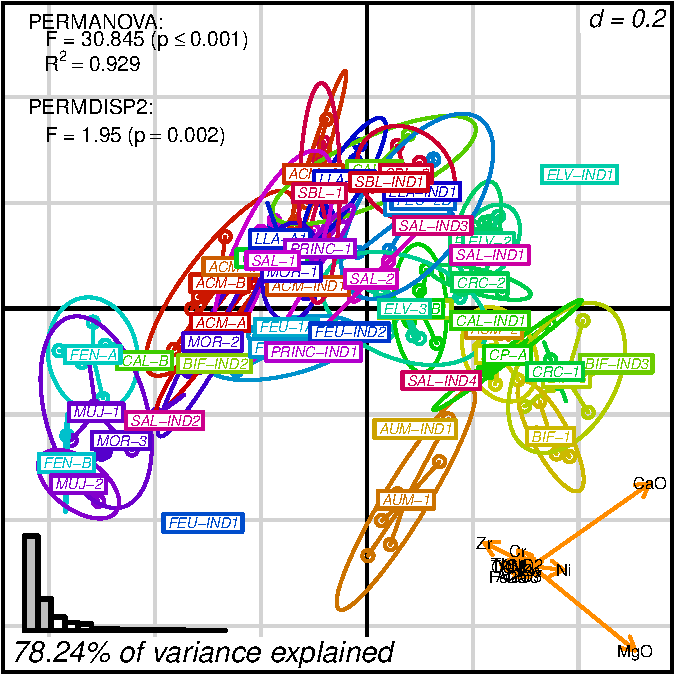
\includegraphics{_main_files/figure-latex/unnamed-chunk-97-1.pdf}
\caption{\label{fig:unnamed-chunk-97}Protocol 1, representing and testing chemical reference groups}
\end{figure}

\pagebreak

Therefore, we can safely interpret positions in terms of having more or less CaO and MgO. For instance, we can classify observations by levels of CaO content and test it against protocol 1 distance matrix and 2D projection:

\begin{Shaded}
\begin{Highlighting}[]
\CommentTok{# Create factor variable containing the classification (5 categories)}
\NormalTok{CaO_level <-}\StringTok{ }\KeywordTok{cut}\NormalTok{(cleanAmphorae}\OperatorTok{$}\NormalTok{CaO[}\OperatorTok{!}\NormalTok{isShipwreck], }\DecValTok{5}\NormalTok{)}

\CommentTok{# Select 5 colours from the 'topo.colors' palette}
\NormalTok{CaO_level_colors <-}\StringTok{ }\KeywordTok{topo.colors}\NormalTok{(}\KeywordTok{nlevels}\NormalTok{(CaO_level))}

\CommentTok{# Test the classification}
\NormalTok{prot1_tests_CaO <-}\StringTok{ }\KeywordTok{test_groups}\NormalTok{(prot1}\OperatorTok{$}\NormalTok{dist_matrix, CaO_level)}
\CommentTok{#> [1] "initiating test batch..."}
\CommentTok{#> [1] "vegan::anosim done."}
\CommentTok{#> [1] "vegan::betadisper done."}
\CommentTok{#> [1] "vegan::permutest done."}
\CommentTok{#> [1] "vegan::adonis done."}
\CommentTok{#> [1] "Test batch completed."}
\end{Highlighting}
\end{Shaded}

\pagebreak

\begin{Shaded}
\begin{Highlighting}[]
\CommentTok{# This is for highlighting CaO arrow}
\NormalTok{arrow_colors <-}\StringTok{ }\KeywordTok{rep}\NormalTok{(}\StringTok{"darkorange"}\NormalTok{, }\KeywordTok{nrow}\NormalTok{(prot1}\OperatorTok{$}\NormalTok{loadings))}
\NormalTok{arrow_colors[}\KeywordTok{row.names}\NormalTok{(prot1}\OperatorTok{$}\NormalTok{loadings) }\OperatorTok{==}\StringTok{ "CaO"}\NormalTok{] <-}\StringTok{ "red"}

\KeywordTok{biplot_2d}\NormalTok{(prot1, }
          \DataTypeTok{groups =}\NormalTok{ CaO_level,}
          \DataTypeTok{group_color =}\NormalTok{ CaO_level_colors,}
          \DataTypeTok{group_star_cex =} \DecValTok{0}\NormalTok{,}
          \DataTypeTok{group_label_cex =} \DecValTok{0}\NormalTok{,}
          \DataTypeTok{show_group_legend =} \OtherTok{TRUE}\NormalTok{,}
          \DataTypeTok{group_legend_title =} \StringTok{"CaO"}\NormalTok{,}
          \DataTypeTok{group_legend_title_pos =} \KeywordTok{c}\NormalTok{(}\FloatTok{0.5}\NormalTok{,}\FloatTok{0.9}\NormalTok{),}
          \DataTypeTok{group_legend_text_cex =} \FloatTok{0.8}\NormalTok{,}
          \DataTypeTok{group_legend_fig =} \KeywordTok{c}\NormalTok{(}\FloatTok{0.7}\NormalTok{,}\FloatTok{0.99}\NormalTok{,}\FloatTok{0.68}\NormalTok{,}\FloatTok{0.95}\NormalTok{),}
          \DataTypeTok{invert_coordinates =} \KeywordTok{c}\NormalTok{(}\OtherTok{TRUE}\NormalTok{, }\OtherTok{TRUE}\NormalTok{),}
          \DataTypeTok{arrow_label_cex =} \FloatTok{0.8}\NormalTok{,}
          \DataTypeTok{arrow_fig =} \KeywordTok{c}\NormalTok{(.}\DecValTok{6}\NormalTok{,.}\DecValTok{95}\NormalTok{,}\DecValTok{0}\NormalTok{,.}\DecValTok{35}\NormalTok{),}
          \DataTypeTok{arrow_label_adj_override =}\NormalTok{ arrows_label_adj,}
          \DataTypeTok{arrow_color =}\NormalTok{ arrow_colors,}
          \DataTypeTok{test_text =}\NormalTok{ prot1_tests_CaO}\OperatorTok{$}\KeywordTok{text}\NormalTok{(prot1_tests_CaO),}
          \DataTypeTok{test_cex =} \FloatTok{0.8}\NormalTok{,}
          \DataTypeTok{test_fig =} \KeywordTok{c}\NormalTok{(}\DecValTok{0}\NormalTok{, }\FloatTok{0.5}\NormalTok{, }\FloatTok{0.65}\NormalTok{, }\FloatTok{.99}\NormalTok{),}
          \DataTypeTok{output_type =} \StringTok{"preview"}\NormalTok{)}
\end{Highlighting}
\end{Shaded}

\begin{figure}
\centering
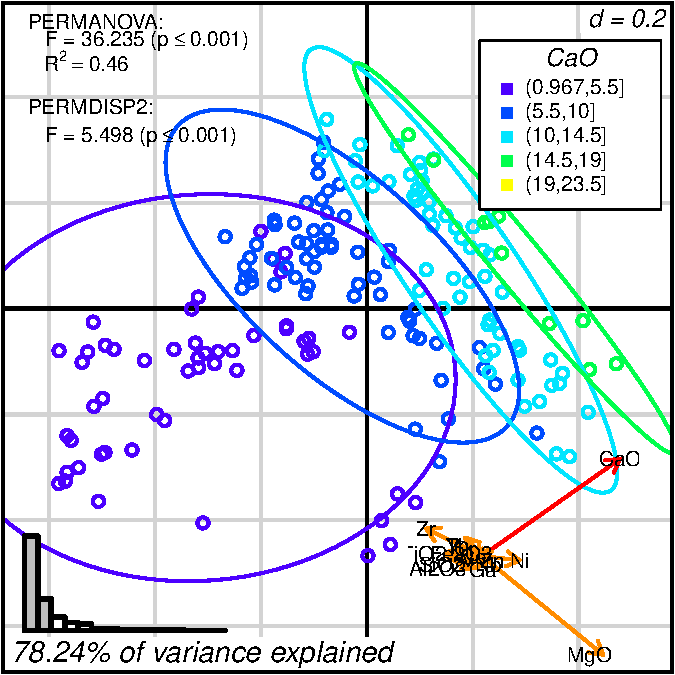
\includegraphics{_main_files/figure-latex/unnamed-chunk-99-1.pdf}
\caption{\label{fig:unnamed-chunk-99}Protocol 1, grouping by level of CaO content}
\end{figure}

\pagebreak

However, interpretation is less straightforward when more than two variables contribute significantly to the total variation. Regarding biplots, such situation implies that a smaller portion of variation is represented, and that several variables are stretch on many directions over the two principal coordinates.

For example, \protect\hyperlink{prot2}{protocol 2} gave us a much worse 2D projection (55.7\%) where fifteen variables are well represented.

\begin{Shaded}
\begin{Highlighting}[]
\CommentTok{# Recover protocol 2a override for variable label positions }
\NormalTok{arrows_label_adj <-}\StringTok{ }\KeywordTok{rbind}\NormalTok{(}\KeywordTok{c}\NormalTok{(.}\DecValTok{5}\NormalTok{,.}\DecValTok{8}\NormalTok{),}\KeywordTok{c}\NormalTok{(.}\DecValTok{5}\NormalTok{,}\DecValTok{1}\NormalTok{),}\KeywordTok{c}\NormalTok{(.}\DecValTok{5}\NormalTok{,}\DecValTok{1}\NormalTok{),}\KeywordTok{c}\NormalTok{(.}\DecValTok{5}\NormalTok{,}\DecValTok{0}\NormalTok{),}\KeywordTok{c}\NormalTok{(.}\DecValTok{5}\NormalTok{,}\DecValTok{1}\NormalTok{),}
                          \KeywordTok{c}\NormalTok{(.}\DecValTok{5}\NormalTok{,}\DecValTok{0}\NormalTok{),}\KeywordTok{c}\NormalTok{(}\DecValTok{0}\NormalTok{,.}\DecValTok{5}\NormalTok{))}
\KeywordTok{row.names}\NormalTok{(arrows_label_adj) <-}\StringTok{ }\KeywordTok{c}\NormalTok{(}\StringTok{"L48"}\NormalTok{,}\StringTok{"L24"}\NormalTok{,}\StringTok{"L5"}\NormalTok{,}\StringTok{"L36"}\NormalTok{,}\StringTok{"S7"}\NormalTok{,}
                                 \StringTok{"S8"}\NormalTok{,}\StringTok{"S11"}\NormalTok{)}

\CommentTok{# This will help us select different arrow colours}
\NormalTok{isDisplayed <-}\StringTok{ }
\StringTok{  }\KeywordTok{row.names}\NormalTok{(prot2a_2d}\OperatorTok{$}\NormalTok{loadings) }\OperatorTok\StringTok{ }\KeywordTok{row.names}\NormalTok{(}
    \KeywordTok{filter_arrows}\NormalTok{(prot2a_2d}\OperatorTok{$}\NormalTok{loadings, }\DataTypeTok{min_dist =} \FloatTok{0.5}\NormalTok{))}
\end{Highlighting}
\end{Shaded}

\pagebreak

\begin{Shaded}
\begin{Highlighting}[]
\NormalTok{biplot2d3d}\OperatorTok{::}\KeywordTok{biplot_2d}\NormalTok{(prot2a_2d,}
                      \DataTypeTok{ordination_method =} \StringTok{"PCoA"}\NormalTok{,}
                      \DataTypeTok{invert_coordinates =} \KeywordTok{c}\NormalTok{ (}\OtherTok{TRUE}\NormalTok{,}\OtherTok{TRUE}\NormalTok{),}
                      \DataTypeTok{xlim =} \KeywordTok{c}\NormalTok{(}\OperatorTok{-}\NormalTok{.}\DecValTok{26}\NormalTok{,.}\DecValTok{35}\NormalTok{),}
                      \DataTypeTok{ylim =} \KeywordTok{c}\NormalTok{(}\OperatorTok{-}\NormalTok{.}\DecValTok{31}\NormalTok{,.}\DecValTok{35}\NormalTok{),}
                      \DataTypeTok{point_type =} \StringTok{"point"}\NormalTok{,}
                      \DataTypeTok{groups =}\NormalTok{ factor_list}\OperatorTok{$}\NormalTok{FabricGroup,}
                      \DataTypeTok{group_color =}\NormalTok{ color_list}\OperatorTok{$}\NormalTok{FabricGroup,}
                      \DataTypeTok{group_label_cex =} \FloatTok{0.6}\NormalTok{,}
                      \DataTypeTok{arrow_mim_dist =} \FloatTok{0.5}\NormalTok{,}
                      \DataTypeTok{arrow_label_cex =} \FloatTok{0.6}\NormalTok{,}
                      \DataTypeTok{arrow_fig =} \KeywordTok{c}\NormalTok{(.}\DecValTok{6}\NormalTok{,.}\DecValTok{95}\NormalTok{,}\DecValTok{0}\NormalTok{,.}\DecValTok{35}\NormalTok{),}
                      \DataTypeTok{arrow_label_adj_override =}\NormalTok{ arrows_label_adj,}
                      \DataTypeTok{subtitle =}\NormalTok{ prot2a_2d}\OperatorTok{$}\NormalTok{sub2D,}
                      \DataTypeTok{test_text =}\NormalTok{ prot2a_tests}\OperatorTok{$}\KeywordTok{text}\NormalTok{(prot2a_tests),}
                      \DataTypeTok{test_cex =} \FloatTok{0.8}\NormalTok{,}
                      \DataTypeTok{test_fig =} \KeywordTok{c}\NormalTok{(}\DecValTok{0}\NormalTok{, }\FloatTok{0.5}\NormalTok{, }\FloatTok{0.65}\NormalTok{, }\FloatTok{.99}\NormalTok{),}
                      \DataTypeTok{fitAnalysis_fig =} \KeywordTok{c}\NormalTok{(}\DecValTok{0}\NormalTok{,.}\DecValTok{7}\NormalTok{,.}\DecValTok{05}\NormalTok{,.}\DecValTok{5}\NormalTok{),}
                      \DataTypeTok{output_type =} \StringTok{"preview"}\NormalTok{)}
\end{Highlighting}
\end{Shaded}

\begin{figure}
\centering
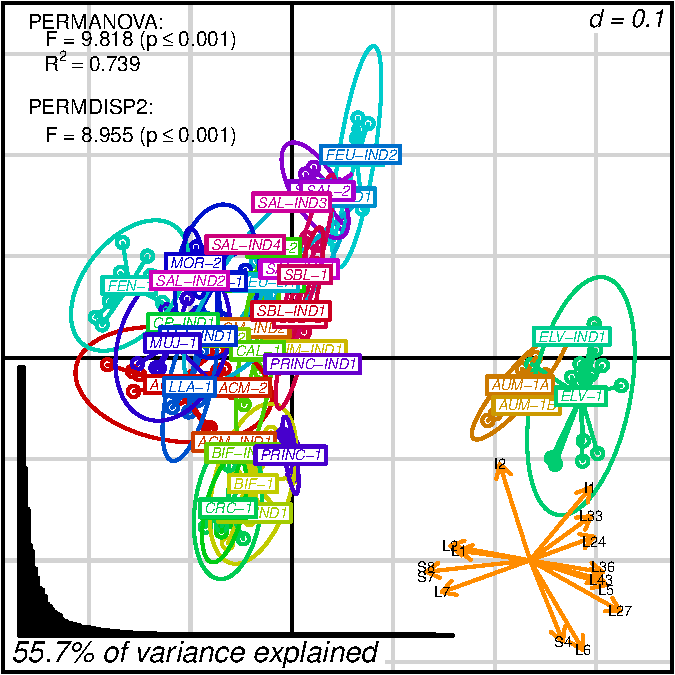
\includegraphics{_main_files/figure-latex/unnamed-chunk-102-1.pdf}
\caption{\label{fig:unnamed-chunk-102}protocol 2a, representing and testing fabric groups}
\end{figure}

\pagebreak

Like in protocol 1, we may want to interpret this projection in terms of a single variable. A obvious candidate is I2 since it is displayed long and quite isolated from other variables.

In this case, I2 (or INCLUS\_ORIENT) is already a factor variable (classification) with 3 categories (plus ``none'' as a missing value). Note that the selected dataset will have cases in only two of those categories.

\begin{Shaded}
\begin{Highlighting}[]
\CommentTok{# You may want to assure that the true }
\CommentTok{# categories are corectly represented:}
\NormalTok{cleanAmphorae <-}\StringTok{ }\KeywordTok{order_petro}\NormalTok{(cleanAmphorae)}

\KeywordTok{levels}\NormalTok{(cleanAmphorae}\OperatorTok{$}\NormalTok{INCLUS_ORIENT[}\OperatorTok{!}\NormalTok{isShipwreck])}
\CommentTok{#> [1] "unparallel"        "slightly parallel" "parallel"         }
\CommentTok{#> [4] "none"}

\CommentTok{# Declare this factor separately as an object for clearness}
\NormalTok{I2 <-}\StringTok{ }\NormalTok{cleanAmphorae}\OperatorTok{$}\NormalTok{INCLUS_ORIENT[}\OperatorTok{!}\NormalTok{isShipwreck]}

\CommentTok{# Select colours from the 'topo.colors' palette}
\NormalTok{I2_colors <-}\StringTok{ }\KeywordTok{topo.colors}\NormalTok{(}\KeywordTok{nlevels}\NormalTok{(I2))}

\CommentTok{# Test the classification}
\NormalTok{prot1_tests_I2 <-}\StringTok{ }\KeywordTok{test_groups}\NormalTok{(prot2a_2d}\OperatorTok{$}\NormalTok{dist_matrix, I2)}
\CommentTok{#> [1] "initiating test batch..."}
\CommentTok{#> [1] "vegan::anosim done."}
\CommentTok{#> [1] "vegan::betadisper done."}
\CommentTok{#> [1] "vegan::permutest done."}
\CommentTok{#> [1] "vegan::adonis done."}
\CommentTok{#> [1] "Test batch completed."}
\end{Highlighting}
\end{Shaded}

\pagebreak

\begin{Shaded}
\begin{Highlighting}[]
\CommentTok{# This is for highlighting I2 arrow}
\NormalTok{arrow_colors <-}\StringTok{ }\KeywordTok{rep}\NormalTok{(}\StringTok{"darkorange"}\NormalTok{, }\KeywordTok{nrow}\NormalTok{(prot2a_2d}\OperatorTok{$}\NormalTok{loadings))}
\NormalTok{arrow_colors[}\KeywordTok{row.names}\NormalTok{(prot2a_2d}\OperatorTok{$}\NormalTok{loadings) }\OperatorTok{==}\StringTok{ "I2"}\NormalTok{] <-}\StringTok{ "red"}
\CommentTok{# filter arrows colours, since not all variables are displayed}
\NormalTok{arrow_colors <-}\StringTok{ }\NormalTok{arrow_colors[isDisplayed]}

\NormalTok{biplot2d3d}\OperatorTok{::}\KeywordTok{biplot_2d}\NormalTok{(prot2a_2d,}
                      \DataTypeTok{ordination_method =} \StringTok{"PCoA"}\NormalTok{,}
                      \DataTypeTok{invert_coordinates =} \KeywordTok{c}\NormalTok{ (}\OtherTok{TRUE}\NormalTok{,}\OtherTok{TRUE}\NormalTok{),}
                      \DataTypeTok{xlim =} \KeywordTok{c}\NormalTok{(}\OperatorTok{-}\NormalTok{.}\DecValTok{26}\NormalTok{,.}\DecValTok{35}\NormalTok{),}
                      \DataTypeTok{ylim =} \KeywordTok{c}\NormalTok{(}\OperatorTok{-}\NormalTok{.}\DecValTok{31}\NormalTok{,.}\DecValTok{35}\NormalTok{),}
                      \DataTypeTok{groups =}\NormalTok{ I2,}
                      \DataTypeTok{group_color =}\NormalTok{ I2_colors,}
                      \DataTypeTok{group_star_cex =} \DecValTok{0}\NormalTok{,}
                      \DataTypeTok{group_label_cex =} \DecValTok{0}\NormalTok{,}
                      \DataTypeTok{show_group_legend =} \OtherTok{TRUE}\NormalTok{,}
                      \DataTypeTok{group_legend_title =} \StringTok{"INCLUS_ORIENT"}\NormalTok{,}
                      \DataTypeTok{group_legend_title_pos =} \KeywordTok{c}\NormalTok{(}\FloatTok{0.5}\NormalTok{,}\FloatTok{0.9}\NormalTok{),}
                      \DataTypeTok{group_legend_text_cex =} \FloatTok{0.8}\NormalTok{,}
                      \DataTypeTok{group_legend_fig =} \KeywordTok{c}\NormalTok{(}\FloatTok{0.6}\NormalTok{,}\FloatTok{0.99}\NormalTok{,}\FloatTok{0.68}\NormalTok{,}\FloatTok{0.95}\NormalTok{),}
                      \DataTypeTok{arrow_mim_dist =} \FloatTok{.5}\NormalTok{,}
                      \DataTypeTok{arrow_label_cex =} \FloatTok{0.8}\NormalTok{,}
                      \DataTypeTok{arrow_fig =} \KeywordTok{c}\NormalTok{(.}\DecValTok{6}\NormalTok{,.}\DecValTok{95}\NormalTok{,}\DecValTok{0}\NormalTok{,.}\DecValTok{35}\NormalTok{),}
                      \DataTypeTok{arrow_label_adj_override =}\NormalTok{ arrows_label_adj,}
                      \DataTypeTok{arrow_color =}\NormalTok{ arrow_colors,}
                      \DataTypeTok{subtitle =}\NormalTok{ prot2a_2d}\OperatorTok{$}\NormalTok{sub2D,}
                      \DataTypeTok{test_text =}\NormalTok{ prot1_tests_I2}\OperatorTok{$}\KeywordTok{text}\NormalTok{(prot1_tests_I2),}
                      \DataTypeTok{test_cex =} \FloatTok{0.8}\NormalTok{,}
                      \DataTypeTok{test_fig =} \KeywordTok{c}\NormalTok{(}\DecValTok{0}\NormalTok{, }\FloatTok{0.5}\NormalTok{, }\FloatTok{0.65}\NormalTok{, }\FloatTok{.99}\NormalTok{),}
                      \DataTypeTok{output_type =} \StringTok{"preview"}\NormalTok{)}
\end{Highlighting}
\end{Shaded}

\begin{figure}
\centering
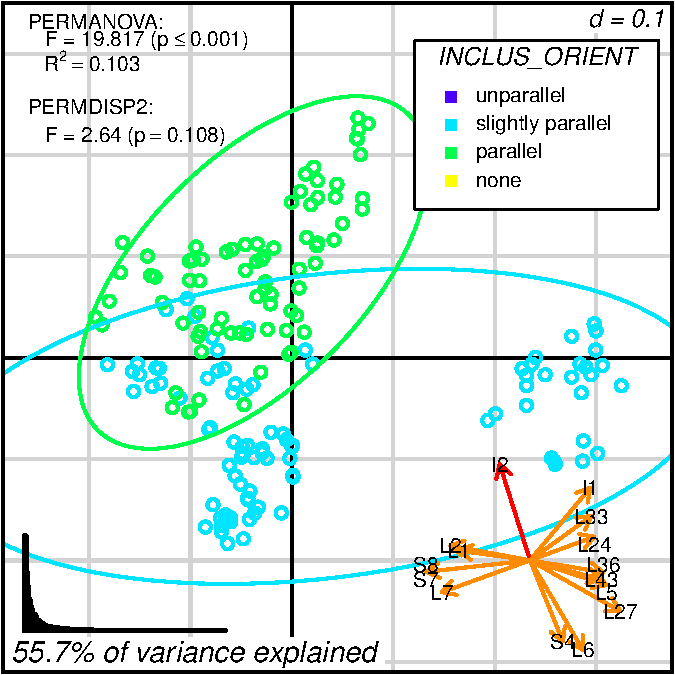
\includegraphics{_main_files/figure-latex/unnamed-chunk-104-1.pdf}
\caption{\label{fig:unnamed-chunk-104}Protocol 2a, grouping by INCLUS\_ORIENT}
\end{figure}

\pagebreak

This kind of reading becomes increasingly difficult when focusing in variables that are not so well aligned, such as L33 (or COAR\_R\_CHERT)

\begin{Shaded}
\begin{Highlighting}[]
\CommentTok{# Declare this factor separately as an object for clearness}
\NormalTok{L33 <-}\StringTok{ }\NormalTok{cleanAmphorae}\OperatorTok{$}\NormalTok{COAR_R_CHERT[}\OperatorTok{!}\NormalTok{isShipwreck]}

\CommentTok{# Select colours from the 'topo.colors' palette}
\NormalTok{L33_colors <-}\StringTok{ }\KeywordTok{topo.colors}\NormalTok{(}\KeywordTok{nlevels}\NormalTok{(L33))}

\CommentTok{# Test the classification}
\NormalTok{prot1_tests_L33 <-}\StringTok{ }\KeywordTok{test_groups}\NormalTok{(prot2a_2d}\OperatorTok{$}\NormalTok{dist_matrix, L33)}
\CommentTok{#> [1] "initiating test batch..."}
\CommentTok{#> [1] "vegan::anosim done."}
\CommentTok{#> [1] "vegan::betadisper done."}
\CommentTok{#> [1] "vegan::permutest done."}
\CommentTok{#> [1] "vegan::adonis done."}
\CommentTok{#> [1] "Test batch completed."}
\end{Highlighting}
\end{Shaded}

\pagebreak

\begin{Shaded}
\begin{Highlighting}[]
\CommentTok{# This is for highlighting L33 arrow}
\NormalTok{arrow_colors <-}\StringTok{ }\KeywordTok{rep}\NormalTok{(}\StringTok{"darkorange"}\NormalTok{, }\KeywordTok{nrow}\NormalTok{(prot2a_2d}\OperatorTok{$}\NormalTok{loadings))}
\NormalTok{arrow_colors[}\KeywordTok{row.names}\NormalTok{(prot2a_2d}\OperatorTok{$}\NormalTok{loadings) }\OperatorTok{==}\StringTok{ "L33"}\NormalTok{] <-}\StringTok{ "red"}
\CommentTok{# filter arrows colours, since not all variables are displayed}
\NormalTok{arrow_colors <-}\StringTok{ }\NormalTok{arrow_colors[isDisplayed]}

\NormalTok{biplot2d3d}\OperatorTok{::}\KeywordTok{biplot_2d}\NormalTok{(prot2a_2d,}
                      \DataTypeTok{ordination_method =} \StringTok{"PCoA"}\NormalTok{,}
                      \DataTypeTok{invert_coordinates =} \KeywordTok{c}\NormalTok{ (}\OtherTok{TRUE}\NormalTok{,}\OtherTok{TRUE}\NormalTok{),}
                      \DataTypeTok{xlim =} \KeywordTok{c}\NormalTok{(}\OperatorTok{-}\NormalTok{.}\DecValTok{26}\NormalTok{,.}\DecValTok{35}\NormalTok{),}
                      \DataTypeTok{ylim =} \KeywordTok{c}\NormalTok{(}\OperatorTok{-}\NormalTok{.}\DecValTok{31}\NormalTok{,.}\DecValTok{35}\NormalTok{),}
                      \DataTypeTok{groups =}\NormalTok{ L33,}
                      \DataTypeTok{group_color =}\NormalTok{ L33_colors,}
                      \DataTypeTok{group_star_cex =} \DecValTok{0}\NormalTok{,}
                      \DataTypeTok{group_label_cex =} \DecValTok{0}\NormalTok{,}
                      \DataTypeTok{show_group_legend =} \OtherTok{TRUE}\NormalTok{,}
                      \DataTypeTok{group_legend_title =} \StringTok{"COAR_R_CHERT"}\NormalTok{,}
                      \DataTypeTok{group_legend_title_pos =} \KeywordTok{c}\NormalTok{(}\FloatTok{0.5}\NormalTok{,}\FloatTok{0.9}\NormalTok{),}
                      \DataTypeTok{group_legend_text_cex =} \FloatTok{0.8}\NormalTok{,}
                      \DataTypeTok{group_legend_fig =} \KeywordTok{c}\NormalTok{(}\FloatTok{0.6}\NormalTok{,}\FloatTok{0.99}\NormalTok{,}\FloatTok{0.68}\NormalTok{,}\FloatTok{0.95}\NormalTok{),}
                      \DataTypeTok{arrow_mim_dist =} \FloatTok{.5}\NormalTok{,}
                      \DataTypeTok{arrow_label_cex =} \FloatTok{0.8}\NormalTok{,}
                      \DataTypeTok{arrow_fig =} \KeywordTok{c}\NormalTok{(.}\DecValTok{6}\NormalTok{,.}\DecValTok{95}\NormalTok{,}\DecValTok{0}\NormalTok{,.}\DecValTok{35}\NormalTok{),}
                      \DataTypeTok{arrow_label_adj_override =}\NormalTok{ arrows_label_adj,}
                      \DataTypeTok{arrow_color =}\NormalTok{ arrow_colors,}
                      \DataTypeTok{subtitle =}\NormalTok{ prot2a_2d}\OperatorTok{$}\NormalTok{sub2D,}
                      \DataTypeTok{test_text =}\NormalTok{ prot1_tests_L33}\OperatorTok{$}\KeywordTok{text}\NormalTok{(prot1_tests_L33),}
                      \DataTypeTok{test_cex =} \FloatTok{0.8}\NormalTok{,}
                      \DataTypeTok{test_fig =} \KeywordTok{c}\NormalTok{(}\DecValTok{0}\NormalTok{, }\FloatTok{0.5}\NormalTok{, }\FloatTok{0.65}\NormalTok{, }\FloatTok{.99}\NormalTok{),}
                      \DataTypeTok{output_type =} \StringTok{"preview"}\NormalTok{)}
\end{Highlighting}
\end{Shaded}

\begin{figure}
\centering
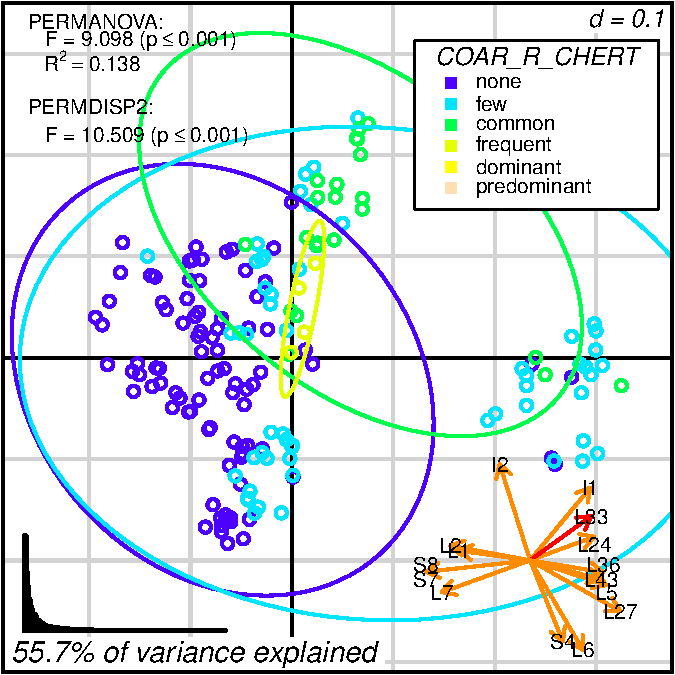
\includegraphics{_main_files/figure-latex/unnamed-chunk-106-1.pdf}
\caption{\label{fig:unnamed-chunk-106}Protocol 2a, grouping by COAR\_R\_CHERT}
\end{figure}

Biplots and ordinal methods (PCA, PCoA, CA, etc.) are exploratory tools that play a game of compromise in order to define the best projections given the whole variance in a dataset. Do not expect them to display patterns that are clear when looking into specific variables. For that kind of analysis, you should use bivariate statistics and graphical displays, such as scatter plots or box plots.


\end{document}
